\documentclass[oneside,senior,etd]{BYUPhys}

%\usepackage[utf8]{inputenc}
\usepackage[russian]{babel}
\usepackage{tikz}
\usepackage{ntheorem}
\usepackage{tabu}
\usepackage{mathtools}
\usepackage{graphicx}
\usepackage{fixltx2e}
\usepackage{caption}
\usepackage{float}
\usepackage{graphicx}
\usepackage{subcaption}
\usepackage{amssymb}
\usepackage{tabularx} % extra features for tabular environment
\usepackage{amsmath}  % improve math presentation
\usepackage{graphicx} % takes care of graphic including machinery
\usepackage[margin=1in,letterpaper]{geometry} % decreases margins
\usepackage{cite} % takes care of citations
\usepackage[final]{hyperref} % adds hyper links inside the generated pdf file


\usetikzlibrary{shapes.geometric,shapes.symbols,positioning,decorations.pathmorphing}

\DeclareMathOperator*{\argmax}{argmax} % thin space, limits underneath in displays
\DeclareMathOperator*{\argmin}{argmin} % thin space, limits underneath in displays
\DeclareMathOperator*{\Motimes}{\text{\raisebox{0.25ex}{\scalebox{0.8}{$\bigotimes$}}}}


\newcommand*\circled[1]{\tikz[baseline=(char.base)]{
            \node[shape=circle,draw,inner sep=2pt] (char) {#1};}}
   
%\hypersetup{
    linktocpage=true,           % ссылки с номера страницы в оглавлении, списке таблиц и списке рисунков
    plainpages=false,           % Forces page anchors to be named by the Arabic form  of the page number, rather than the formatted form
    colorlinks,                 % ссылки отображаются раскрашенным текстом, а не раскрашенным прямоугольником, вокруг текста
    linkcolor=blue,      % цвет ссылок типа ref, eqref и подобных
    citecolor=blue,      % цвет ссылок-цитат
    urlcolor=blue,        % цвет гиперссылок
    pdflang={ru}
}
%\graphicspath{{./images/}}
\fixmargins
\oneandhalfspace

\DeclareMathOperator*{\argmax}{argmax} % thin space, limits underneath in displays
\DeclareMathOperator*{\argmin}{argmin} % thin space, limits underneath in displays
\DeclareMathOperator*{\Motimes}{\text{\raisebox{0.25ex}{\scalebox{0.8}{$\bigotimes$}}}}

\newcommand\myeq{\mathrel{\overset{\makebox[0pt]{\mbox{\normalfont\tiny\sffamily def}}}{=}}}

\usepackage[utf8]{inputenc}
\usepackage{rotating} 

\usepackage[english, russian]{babel}
\usepackage{amsfonts} % Пакеты для математических символов и теорем
\usepackage{amstext}
\usepackage{amssymb}
\usepackage{amsthm}
\usepackage{graphicx} % Пакеты для вставки графики
\usepackage{subfig}
\usepackage{color}
\usepackage[unicode]{hyperref}
\usepackage[nottoc]{tocbibind} % Для того, чтобы список литературы отображался в оглавлении
\usepackage{algorithmic} % Для записи алгоритмов в псевдокоде
\usepackage{algorithm}
\usepackage{verbatim} % Для вставок заранее подготовленного текста в режиме as-is
\usepackage{listings}

\usepackage{commath}
\newcommand\Tau{\mathcal{T}}
\newcommand{\R}{\mathbb{R}}

\Chair{Кафедра Исследования Операций}
\Lab{~}
\Year{2019}
  \Month{Июнь}
  \City{Москва}
  \AuthorText{Автор}
  \Author{Кононов Сергей Владиславович}
  \AuthorEng{Kononov Sergey}
  \AcadGroup{411}

  \TitleTop{Исследование модельной игры преподавателя и студента}
  \TitleBottom{с применением свёртки Гермейера у студента} % leave empty if you don't need it
  \TitleTopEng{Research into teacher-student model game with use of}
  \TitleBottomEng{Germeyer's scalarization for student} % leave empty if you don't need it  
  \docname{Выпускная квалификаионная работа}
  \Advisor{Новикова Наталья Михайловна}  
  \AdvisorDegree{д-р физ.-мат. наук\\}

\Abstract{
В данной работе исследуются вопрос параметризации и аппроксимации множества Парето при помощи обратной логической свертки ($O$$\Lambda$$C$).
Проводится обзор методов решения для частной задачи на языке программирования Python.
}
\AbstractEng{Abstract}


%%%% DON'T change this. It is here because .sty does not support cyrillic cp properly %%%%
\University{Московский Государственный Университет имени М.В.Ломоносова}
\Faculty{Факультет Вычислительной Математики и Кибернетики}
\GrText{группа}
\AdvisorText{Научный руководитель}
\AbstractText{Аннотация}

\begin{document}
\fixmargins
\makepreliminarypages

\oneandhalfspace

\tableofcontents

\tableofcontents
\clearpage

\cite{blackwell}

%\section{Введение}
\begin{flushleft}

\qquad В работе рассматриваются различные способы решения модельной задачи которая
представляет собой игру двух лиц с противоположными интересами и двумерной
функцией выигрыша. Для решения задачи применяется модифицированный
метод свёрток предложенный Л.С. Шепли, который как правило используется в
подобных задачах.

\subsection{Игровая модель}

\qquad Рассматриваются два игрока - Студент, далее обозначается \textbf{С},
и Преподаватель, далее обозначается \textbf{П}, которые имеют противоположные интересы.
Критерий интересов составляют две велечины, первая из которых является эффективностью
работы \textbf{С} в научной сфере, а второй его эффективностью на подработке.

\qquad \textbf{С} выбирает долю $x$ рабочего времени, которую он тратит на подготовку
диплома, оставшееся рабочее время $1-x$ он тратит на подработку. Считается, что производительность \textbf{С} при любых занятий падает с увеличением 
отводимого на них времени, эффективность труда \textbf{С} зададим функцией $\sqrt{x}$
и $\sqrt{1-x}$ соответственно. \textbf{С} может распределять свое время между двумя 
видами деятельности, т.е. имеет множетсво стратегий $x\in X = \{0, 1\}$, 
причём он может использовать смешанные стратегии.

\qquad \textbf{П} выбирает - отностится к \textbf{С} требовательно, способствую 
написанию диплома и мешая подработке или же не обращать на него внимания не 
мешая подработке и не помогая с дипломом. \textbf{П} имеет множество стратегий 
$y \in Y=\{1, 2\}$, причём тоже может использовать смешаные стратегии.

\vspace{5mm}
\qquad Получаем следующий функциональный критерий:

$$
F(x, y)=
\big(f_1(x,y), f_2(x,y)\big) =
\Big(
	\frac{y\sqrt{x}}2,
	\frac{\sqrt{1-x}}y
\Big)
$$

\qquad \textbf{П} стремится минимизировать (выборая $y \in Y = \{1,2\}$)
критерий $F(x, y)$, а игрок \textbf{С} - максимизировать
 (выбирая $x \in X=[0,1]$).

\vspace{5mm} 
Задачу можно представить в виде многокритериальную игру двух лиц 
с противоположными интересамив 

\begin{equation}
	\bigg \langle F(x,y), X, Y \bigg \rangle, \; y \in Y=\{1, 2\}, \; x \in {X}=[0, 1]
	\label{eq:mc_game}
\end{equation}

\newtheorem{Def}{Определение}
\begin{Def}
	Допустимое решение $\hat{x}\in{X}$ называется 
	строго эффективным (эффективным по Слейтеру) для задачи
	\begin{equation}
		\max\limits_{x \in X} F(x)=({f}_1(x),\ldots, {f}_n(x))
		\label{eq:mc_problem}
	\end{equation}
	если \textbf{не} существует $x\in{X}$ такого, что 
	$f_k(x)>f_k(\hat{x})$ для всех $k=\{1,...,n\}$. Множетсво всех эффективных по
	Слейтеру решений называается \textit{множеством Слейтера} задачи \eqref{eq:mc_problem}.
\end{Def}

Для задачи \eqref{eq:mc_game} введеём следующие частные случаи:

\begin{gather*}
	S_x(y^*) \textrm{ - множество Слейтера задачи } \max\limits_{x \in X} F(x, y^*) \\
	S_y(x^*) \textrm{ - множество Слейтера задачи } \min\limits_{y \in Y} F(x^*, y)
\end{gather*}

\begin{Def}
	Решением\footnote {
	Согласно \textit{Blackwell D.} An analog of the minimax theorem for
    vector payoffs // Pac. J. of Math. 1956. No 6.
	} 
	\eqref{eq:mc_game} является множество точек $(x^*, y^*)$ таких, что
    $x^* \in Х S_x(y^*) $ и $ y^*  \in S_y (x^*)$, 
\end{Def}

\vspace{5mm}

\qquad Для параметризации множеств Слейтера будем использовать метод свёрток.
Он заключается в том, что задача $\max\limits_{x \in X} F(x)$ заменяется параметрическим 
семейством скалярных задач $\max\limits_{x \in X} C(\{f_i\}, \lambda, x)$, \newline 
где $C$ – функция свертки частных критериев $\{f_i\}_{i=1}^m$ задачи 
\eqref{eq:mc_problem} в единый скалярный критерий, $\lambda$ – параметр свертки. 

\begin{Def}
	Линейной свёрткой с параметром $\lambda$ для функции критериев задачи
	\eqref{eq:mc_problem} называется функция:
	\begin{equation}
		L(\{f_i\}, \lambda, x)=\sum_{i=1}^{m} \lambda_i f_i \textrm{, где }
		\lambda \in \Lambda =\{\lambda_i \geq 0 | \sum_{i=1}^n \lambda_i =1 \},
	\end{equation}

	свёрткой Гермейера или обратной логической свёрткой с параметром $\mu$ для 
	функции критериев задачи \eqref{eq:mc_problem} называется функция:
	\begin{equation}
		G(\{f_i\}, \mu, x)=
		\min\limits_{i: \mu_i > 0} \frac{f_i}{\mu_i} \textrm{, где }
		\mu \in M =\{\mu_i \geq 0 | \sum_{i=1}^n \mu_i =1 \}.
	\end{equation}
\end{Def}

\qquad В случае конечных $X$ и $Y$ Шепли свел [4] описание данного множества к
семейству задач поиска значений скалярных игр с функциями выигрышей – 
ЛС частных критериев при произвольном наборе весовых коэффициентов, 
своих у каждого игрока. Применение линейной свертки в многокритериальных 
задачах обосновывается леммой Карлина

\newtheorem{Th}{Теорема}
\begin{Th}[Карлин (5)]
	Пусть $x_0$ – эффективная точка,
    Тогда существуют неотрицательные числа $\lambda_1,…,\lambda_m$ такие, 
    что $\sum_{i=1}^m \lambda_i=1$ и $x_0$ является точкой максимума функции  
    $L(x) =\sum_{j=1}^m \lambda_j f^j(x)$ 
\end{Th}

\qquad Гермейером была предложена свертка, которая также аппроксимирует 
множество Слейтера. В работе используется ее модификация -
обратная логическая свертка, она отличается тем, что веса стоят в знаменателе.

\begin{Th}[Гермейер (5)]
    Пусть $x_0$ – эффективная точка, причем $f^i(x_0)>0$ для всех 
    $i=1,…,m.$
    Тогда существуют положительные числа $\lambda_1,…,\lambda_m$ такие, 
    что $\sum_{i=1}^m \lambda_i=1$ и $x_0$ является точкой максимума функции  
    $G(x) =\min \limits_{1 \leqslant j \leqslant m} \lambda_j f^j(x)$.
\end{Th}

Рассмотрим случай, когда \textbf{С} использует обратную логическую свертку,
с парамером $\mu$, a \textbf{П} использует линейную
свертку с параметром $\lambda$. Тогда множество оптимальных решений:

\begin{gather*}
	\begin{cases}
		x^*=\arg \max \limits_{x}   G(\{f_1, f_2\}, \mu, x, y^*) \\
		y^*=\arg \min \limits_{y}   L(\{f_1, f_2\}, \lambda, x^*, y)
	\end{cases}
\end{gather*}

Поскольку игроки используют смешанные стратегии т.е. распределения вероятностей
$\rho_x(x)$ и $\rho_y(y)$ над чистыми стратегиями $x \in X$ и $y \in Y$. 
Далее каждый игрок осредняет свою функцию выигрыша по стратегиям противника

$$ \overline G(\{f_1, f_2\}, \mu, q, p) = 
\iint \limits_{PQ} G(\{f_1, f_2\}, \mu, q, p) \rho_x(x) \rho_y(y)dxdy$$
$$ \overline L(\{f_1, f_2\}, \lambda, q, p) = 
\iint \limits_{PQ} L(\{f_1, f_2\}, \lambda, q, p) \rho_x(x) \rho_y(y)dxdy$$



\begin{Def}
	Пара стратегий $(p^0, q^0)$ называется оптимальными, если для некоторых 
	$\lambda$, $\mu$ верно:
	\begin{equation}
		\begin{cases} 
		p^0(q^0, \lambda) = \argmin\limits_{p \in P} \overline L(p, q^0, \lambda) \\ 
		q^0(p^0, \mu) = \argmin\limits_{q \in Q} \overline G(p^0, q, \mu) \\
	\end{cases}
\end{equation}
\end{Def}

Мы будем рассматривать конечную игру \textbf{C --- П}, полученную из исходной 
заменой множества $X=[0,1]$ конечным множеством точек

$$X^T = \{
	0, \; \frac{1}{T}, \; \frac{2}{T}, \; \ldots, \; \frac{T-1}{T}, \; 1
\}, \;\; T \in \mathbb{N}$$

В работе исследуются случаи $T=1$: $X^1=\{0, 1\}$, 
и $T=2$: $X^2=\{0, \frac{1}{2} ,1\}$



\end{flushleft}
%\include{include/game_model}
%\section{Постановка задачи (значение параметра T=1)}

\subsection{Игровая модель}

\qquad Рассматриваются два игрока - Студент, далее обозначается \textbf{С},
и Преподаватель, далее обозначается \textbf{П}, которые имеют противоположные интересы.
Критерий интересов составляют две велечины, первая из которых является эффективностью
работы \textbf{С} в научной сфере, а второй его эффективностью на подработке.

\textbf{С} выбирает долю $x$ рабочего времени, которую он тратит на подготовку
диплома, оставшееся рабочее время $1-x$ он тратит на подработку. Считается, что производительность \textbf{С} при любых занятий падает с увеличением 
отводимого на них времени, эффективность труда \textbf{С} зададим функцией $\sqrt{x}$
и $\sqrt{1-x}$ соответственно. \textbf{С} может распределять свое время между двумя 
видами деятельности, т.е. имеет множетсво стратегий $x\in X = \{0, 1\}$, 
причём он может использовать смешанные стратегии.

\textbf{П} выбирает - отностится к \textbf{С} требовательно, способствую 
написанию диплома и мешая подработке или же не обращать на него внимания не 
мешая подработке и не помогая с дипломом. \textbf{П} имеет множество стратегий 
$y \in Y=\{1, 2\}$, причём тоже может использовать смешаные стратегии.

\vspace{5mm}
Получаем следующий функциональный критерий:

\begin{equation}
	F(x, y)=
	\big(f_1(x,y), f_2(x,y)\big) =
	\Big(
		\frac{y\sqrt{x}}2,
		\frac{\sqrt{1-x}}y
	\Big)
	\label{eq:player_criterion}
\end{equation}

\qquad \textbf{П} стремится минимизировать (выборая $y \in Y = \{1,2\}$)
критерий $F(x, y)$, а игрок \textbf{С} - максимизировать
 (выбирая $x \in X=[0,1]$).

\vspace{5mm} 
Задачу можно представить в виде многокритериальную игру двух лиц 
с противоположными интересамив 

\begin{equation}
	\bigg \langle F(x,y), X, Y \bigg \rangle, \; y \in Y=\{1, 2\}, \; x \in {X}=[0, 1]
	\label{eq:mc_game}
\end{equation}

\subsection{Постановка зададчи}

Сначала рассмотри случай с параметром $T=1$. Тогда множество $X=\{0, 1\}$.
Игроки используют смешанные стратегии т.е. распределение над своими чистыми стратегиями.
Чистыми стратегиями игроков \textbf{С} и \textbf{П} являются $X=\{0, 1\}$ и $Y=\{1,2\}$ 
соответсвенно. Эти множества дискретны, поэтому распределения задаются в виде векторов 
вида: 

$$(p_1, p_2) \in P = \{(p_1, p_2) \in R_+^2 \; | \; p_1 + p_2 = 1)$$

Множество $Q=P$, введено для наглядности. 
Смешанные стратеги игроков \textbf{С} и \textbf{П} будем обозначать
$q=(q_0,q_1) \in Q$ и $p=(p_0,p_1) \in P$ соответсвенно, причём:

\begin{equation}
\begin{tabu} to 0.9 \textwidth {X[c] X[c]}
	$P(X=0)=q_0$ & $P(Y=1)=p_0$ \\
	$P(X=1)=q_1$ & $P(Y=2)=p_1$ \
	\\
	\end{tabu}	
\label{eq:probability_1}
\end{equation}

Введём обозначения $q := q_1$ и $p := p_1$, тогда $q_0 = 1-q$ и $p_0 = 1 - p$. 
Игрок \textbf{С} использует смешаную стратегию  $(q_0,q_1)$, тогда
его векторный критерий \eqref{eq:player_criterion} приобретает вид: 

$$
	F_\textrm{C}(q,y)=
	\big \langle
		q_0\frac{y\sqrt{0}}{2} + 
		q_1\frac{y\sqrt{1}}{2};
		q_0\frac{\sqrt{1}}{y} +
		q_1\frac{\sqrt{0}}{y}
	\big \rangle 
	= 	
	\big \langle
		\frac{q_1y}{2};
		\frac{q_0}{y}
	\big \rangle 
$$

Игрок \textbf{П} использует смешаную стратегию  $(p_0,p_1)$, тогда
его векторный критерий \eqref{eq:player_criterion} приобретает вид: 

\begin{gather*}
	F_\textrm{П}(x,p)=
	\big \langle 
		(1-p)\frac{1 \cdot \sqrt{x}}{2} + p \frac{2 \cdot \sqrt{x}}{2}; \;
		(1-p)\frac{\sqrt{1-x}}{1}+p\frac{\sqrt{1-x}}{2} 
	\big \rangle=
	\\
	=\frac{1}{2}
	\big \langle
		(p+1)\sqrt{x}; \;
		(2-p)\sqrt{1-x}
	\big \rangle
\end{gather*}
	
\vspace{5mm}

Далее игрок \textbf{С} использует \textit{обратную логическую свёртку}
\eqref{eq:germeyer_scalarization}:

$$
	G(y, q, \mu) = 
	\min \limits_{i: \mu_i > 0} \{\frac{q_1y}{2\mu_0};\frac{q_0}{y\mu_1}\},
$$

a игрок \textbf{П} использует \textit{линейную свёртку}
\eqref{eq:linear_scalarization}:

$$
	L(p, x, \lambda) = 
	\lambda_0 (p+1)\sqrt{x} + \lambda_1 (2-p)\sqrt{1-x}
$$

После чего игрок \textbf{С} осредняет свёртку критерия по стратегиям игрока \textbf{П},
т.е. по переменной $y$:

$$
	\overline G(p,q,\mu)=
	p\min{\{\frac{q}{\mu};
	\frac{1-q}{2(1-\mu)}\}}
	+(1-p)\min\{\frac{q}{2\mu};\frac{1-q}{1-\mu}\},
$$

а игрок \textbf{П} осредняет свёртку критерия по стратегиям игрока \textbf{С},
т.е. по переменной $x$:

$$
	\overline L(p, q, \lambda) =
	\frac{1}{2}\big \{q(3\lambda+p-2)+(2-p)(1-\lambda)\big \}.
$$

Мы установили функции выигрыша игроков. Теперь задачу можно формализовать и представить
как семейство игр двух игроков в нормальный форме:

$$
	\bigg \langle 
		\{\textrm{\textbf{С}, \textbf{П}}\},		
		\{Q, \: P\},		
		\{\overline L(p,q,\lambda), - \overline G(p,q,\mu) \}
	\bigg \rangle 
	, \; (\lambda, \mu) \in \Lambda \times  M
$$

Для нас представляет интерес множество оптимальных точек \eqref{def:optimal_strategy}.
%\section{Множество оптимальных стратегий}

Для поиска оптимальных стратегий сначала необходимо найти точки максимума и минимума 
функций выигрыша \textbf{С} и \textbf{П} соответсвенно:

$$
	q^*(p, \mu) = \arg \max \limits_{q \in Q} \overline G(p, q, \mu)
	\textrm{ и }
	p^*(q, \lambda) = \arg \min \limits_{p \in P} \overline L(p, q, \lambda).
$$

Из статьи \cite{novikova} следует, что:

\begin{equation}
	p^*(q, \lambda)=
	\arg \min \limits_{p \in P} \overline L(p, q, \lambda) =
	\begin{cases}
		0, & q > 1 - \lambda \\
		1, & q < 1 - \lambda \\
		[0,1], & q = 1 - \lambda
	\end{cases}
	\label{eq:argmin_L_1}
\end{equation}

Из пункта \textbf{[ещё не написано]} следует, что
\begin{equation}
	q^*(p, \mu) = \arg \max \limits_{q \in Q} \overline G(p, q, \mu) =
	\begin{cases}
		\dfrac{\mu}{2 - \mu}, & p \geqslant 1 - \mu \\
		\dfrac{2\mu}{1 + \mu}, & p \leqslant 1 -\mu \\
	\end{cases}
	\label{eq:argmax_G_1}
\end{equation}

Докажем утверждение характерезующее множество оптимальных пар данной игры.

\newtheorem{State}{Утверждение}\label{State:opt_strat_1}
\begin{State}
	Любая пара $(p^*, q^*) \in [0, 1]^2$ является оптимальной, т.е.  
	$\forall \; (p^*, q^*) \in [0, 1]^2 \; \exists \; 
	(\mu, \lambda) \in M \times \Lambda$
	такие, что верно \eqref{def:optimal_strategy}.
\end{State}


\textbf{Доказательство}

Зафиксируем некоторую пару  $(p^*, q^*) \in [0, 1]^2$ и найдём такие 
$\hat \mu (p^*, q^*) \in M$ и $\hat \lambda (p^*, q^*) \in \Lambda$ 
что верно \eqref{def:optimal_strategy} т.е. что пара стратегий является оптимальной.

\textbf{(1)} Определим $\hat \lambda(p^*, q^*)$ и покажем что 
$p^* \in \arg \min \limits_{p \in P} \overline L(p, q^*, \hat \lambda)$.
Возьмём $\hat \lambda := 1 - q^*$ тогда поскольку 
$\arg \min\limits_{p \in P} \overline L(p, q^*, \hat \lambda) = [0,1]$ 
при $ q^* = 1 - \hat \lambda$, 
то $p^* \in \arg \min \limits_{p \in P} \overline L(p, q^*, \hat \lambda)$.

\textbf{(2)} Определим $\hat \mu(p^*, q^*)$ и покажем что 
$q^* \in \arg \max \limits_{q \in Q} \overline G(p^*, q, \hat \mu) $.
По имеющемуся $q^*$ решим уравнения $\dfrac{\mu}{2 - \mu}=q^*$ и
$\dfrac{2 \mu}{1 + \mu}=q^*$, относительно переменной $\mu$:

$$
	q^*=\dfrac{2 \mu}{1 + \mu} \Rightarrow \mu = \frac{q^*}{2 - q^*} \qquad \qquad
	q^*=\dfrac{\mu}{2 - \mu} \Rightarrow \mu = \frac{2 q^*}{1 + q^*}
$$

Введём обозначения $\mu_1(q) = \dfrac{q}{2 - q}$ и 
$\mu_2(q) = \dfrac{2 q}{1 + q}$. Заметим, что при $q^* \in [0, 1]$ 
верно $0 \leqslant \mu_2(q^*) \leqslant \mu_1(q^*) \leqslant 1$.
В таком случае поскольку $1 - p^* \in [0, 1]$, то при фиксированных переменных 
$(p^*, q^*)$ будет реализован один и только один из 3-х вариантов:

\textbf{(a)}
$1 - p^* \leqslant \mu_2(q^*)$, т.е.  $1 - p^* \leqslant \dfrac{q^*}{2 - q^*}$.
Возьмём $\hat \mu := \mu_1 = \dfrac{2 q^*}{1 + q^*}$.

Действительно, при таком выборе $\hat{\mu}$ имеем: 
\begin{gather*}
	1 - p^* \leqslant \mu_2 \leqslant \mu_1 = \hat \mu \Rightarrow
	p^* \geqslant 1 - \hat \mu \Rightarrow 
	\\	
	\Rightarrow \arg \max \limits_{q \in Q} \overline G(p^*, q, \hat \mu) =
	\dfrac{\hat{\mu}}{2-\hat{\mu}} =
	\dfrac{\dfrac{2 q^*}{1 + q^*}}{2 - \dfrac{2 q^*}{1 + q^*}} =
	q^*
\end{gather*} 


\textbf{(b)}
$\mu_2(q^*) < 1-p^* \leqslant \mu_1(q^*)$, т.е.  
$\dfrac{q^*}{2 - q^{*}} < 1 - p^* \leqslant \dfrac{2 q^*}{1 + q^*}$.
Возьмём $\hat \mu := \mu_1 = \dfrac{2 q^*}{1 + q^*}$.
Действительно, при таком выборе $\hat \mu$ имеем:

\begin{gather*}
	1 - p^* \leq \mu_1 = \hat \mu 
	\; \Rightarrow \;
	p^* \geqslant 1 - \hat \mu \Rightarrow 
	\\
	\Rightarrow  \arg \max \limits_{q \in Q} \overline G(p^*, q, \hat \mu) =
	\dfrac{\hat \mu}{2 - \hat \mu} =
	\dfrac{\dfrac{2 q^*}{1 + q^*}}{2 - \dfrac{2 q^*}{1 + q^*}}=
	q^* \Rightarrow
\end{gather*} 



\textbf{(c)} 
$\mu_1(q^*) < 1 - p^*$ т.е. $\dfrac{2 q^*}{1 + q^*} < 1 - p^*$.
Возьмём $\hat \mu := \mu_2 = \dfrac{q^*}{2 - q^*}$
Действительно, при таком выборе $\hat \mu$ имеем:

\begin{gather*}
	1 - p^* > \mu_1 \geqslant \mu_2 = \hat \mu \Rightarrow
	p^* \leqslant 1 - \hat \mu \Rightarrow 
	\\	
	\Rightarrow \arg \max \limits_{q \in Q} \overline G(p^*, q, \hat \mu) =
	\dfrac{2 \hat \mu}{1 + \hat \mu} =
	\dfrac{2 \dfrac{q^*}{2 - q^*}}{1 + \dfrac{q^*}{2 - q^*}} =
	q^*.
\end{gather*}

Теперь для любой точки $(p^*,q^*) \in [0,1]^2$ можем указать
$(\hat \mu(p^*,q^*), \hat \lambda(p^*,q^*))$ такие, что верно \eqref{def:optimal_strategy},
а именно:
 
$$
(\hat \mu(p^*,q^*), \hat \lambda(p^*,q^*)) = 
\begin{cases}
	\Big(\dfrac{q^*}{2 - q^*}, \: 1 - q^* \Big), &
	\dfrac{2 q^*}{1 + q^*} < 1 - p^*
	\\
	\Big(\dfrac{2 q^*}{1 + q^*}, \: 1 - q^* \Big), &
	1 - p^* \leqslant \dfrac{q^*}{2 - q^*}
	\\
	\Big(\dfrac{2 q^*}{1 + q^*}, \: 1 - q^*\Big), & 	
	\dfrac{q^*}{2 - q^{*}} < 1 - p^* \leqslant \dfrac{2 q^*}{1 + q^*}
\end{cases}
$$

\textbf{Утверждение доказано.}

%\section{Подробное рассмотрение множества оптимальных стратегий}

Для каждой пары параметров $(\hat \mu, \hat \lambda)$ найдём множество
соответсвующих оптимальных пар 
$(p^*(\hat \mu, \hat \lambda), q^*(\hat \mu, \hat \lambda)) \in P \times Q$. 
Рассмотрим все возможные сочетания значений для $p^*$ и $q^*$ в системах 
\eqref{eq:argmin_L_1} \eqref{eq:argmax_G_1}, что даст нам 6 следующих систем:

\hspace{5mm}

	\textit{Учтём, что переменные $p, q, \mu$ и $\lambda$ определены на отрезке $[0, 1]$.}
	
%---------------------------1------------------------
\textbf{(1)}
$$
	\begin{cases}
		p^* = 0 \\
		q^* = \dfrac{\mu}{2 - \mu} \\
		q^* > 1 - \lambda \\
		p^* + \mu - 1 \geqslant 0 \\
	\end{cases}
	\quad \sim \quad
	\begin{cases}
		p^* = 0 \\
		q^* = \dfrac{\mu}{2 - \mu} \\
		\dfrac{\mu}{2 - \mu} > 1 - \lambda \\
		\mu \geqslant 1 \quad \Rightarrow \quad \mu = 1 \\
	\end{cases}
	\quad \sim \quad
	\begin{cases}
		p^* = 0 \\
		q^* = 1 \\
		\lambda > 0 \\
		\mu = 1
	\end{cases}
$$

Значит при $\mu = 1$  и $\lambda \in (0,1]$ имеем следующие оптимальные пары:
$(p^*, q^*) \in (0, 1)$

%---------------------------2------------------------
\hspace{5mm}

\textbf{(2)}
$$
	\begin{cases}
		p^* = 0 \\
		q^* = \dfrac{2\mu}{1+\mu} \\
		q^* > 1 - \lambda \\
		p^* + \mu - 1 \leqslant 0 \\
	\end{cases}
	\quad \sim \quad
	\begin{cases}
		p^* = 0 \\
		q^* = \dfrac{2\mu}{1+\mu} \\
		\dfrac{2\mu}{1+\mu} > 1 - \lambda \\
		\mu \leqslant 1
	\end{cases}
	\quad \sim \quad
	\begin{cases}
		p^* = 0 \\
		q^* = \dfrac{2\mu}{1+\mu} \\
		\lambda > \dfrac{1-\mu}{1+\mu} \\
		\mu \leqslant 1
	\end{cases}
$$

Значит при $\mu \in [0, 1]$ и $\lambda \in (\frac{1-\mu}{1+\mu}, 1]$
имеем следующие оптимальные пары
$(p^*, q^*) \in (0, \dfrac{2\mu}{1 + \mu})$

%---------------------------3------------------------
\hspace{5mm}

\textbf{(3)}
$$
	\begin{cases}
		p^* = 1 \\
		q^* = \dfrac{\mu}{2-\mu} \\
		q^* < 1 - \lambda \\
		p^* + \mu - 1 \geqslant 0 \\
	\end{cases}
	\quad \sim \quad
	\begin{cases}
		p^* = 1 \\
		q^* = \dfrac{\mu}{2-\mu} \\
		\dfrac{\mu}{2-\mu} < 1 - \lambda \\
		\mu \geqslant 0
	\end{cases}
	\quad \sim \quad
	\begin{cases}
		p^* = 1 \\
		q^* = \dfrac{\mu}{2-\mu} \\
		\lambda < 2\dfrac{1-\mu}{2-\mu} \\
		\mu \geqslant 0
	\end{cases}
$$

Значит при $\mu \in [0, 1]$ и $\lambda \in [0, 2\frac{1-\mu}{2-\mu})$
имеем следующие оптимальные пары
$ (p^*, q^*) \in (1, \frac{\mu}{2 - \mu})$

%---------------------------4------------------------
\hspace{5mm}

\textbf{(4)}
$$
	\begin{cases}
		p^* = 1 \\
		q^* = \dfrac{2\mu}{1+\mu} \\
		q^* < 1 - \lambda \\
		p^* + \mu - 1 \leqslant 0 \\
	\end{cases}
	\quad \sim \quad
	\begin{cases}
		p^* = 1 \\
		q^* = \dfrac{2\mu}{1+\mu} \\
		\dfrac{2\mu}{1+\mu} < 1 - \lambda \\
		\mu \leqslant 0 \quad \Rightarrow \quad \mu = 0 \\
	\end{cases}
	\quad \sim \quad
	\begin{cases}
		p^* = 1 \\
		q^* = 0 \\
		\lambda < 1 \\
		\mu = 0
	\end{cases}
$$

Значит при $\mu=0$ и $\lambda \in [0, 1)$ имеем следующие оптимальные пары
$ (p^*, q^*) \in (1, 0)$

%---------------------------5------------------------
\hspace{5mm}

\textbf{(5)}
$$
	\begin{cases}
		p^* \in [0, 1] \\
		q^* = \dfrac{\mu}{2-\mu} \\
		q^* = 1 - \lambda \\
		p^* + \mu - 1 \geqslant 0 \\
	\end{cases}
	\quad \sim \quad
	\begin{cases}
		p^* \in [0, 1] \\
		q^* = \dfrac{\mu}{2-\mu} \\
		\dfrac{\mu}{2-\mu} = 1 - \lambda \\
		p^* \geqslant 1 - \mu \\
	\end{cases}
	\quad \sim \quad
	\begin{cases}
		p^* \in [1 - \mu, 1] \\
		q^* = \dfrac{\mu}{2-\mu} \\
		\lambda = 2\dfrac{1-\mu}{2-\mu} \\
	\end{cases}
$$

Значит при $\mu \in [0, 1]$ и $\lambda = 2\dfrac{1 - \mu}{2 - \mu}$ 
имеем следующие оптимальные пары
$ (p^*, q^*) \in [1 - \mu, 1] \times  \{ \frac{\mu}{2 - \mu}\}$

%---------------------------6------------------------
\hspace{5mm}

\textbf{(6)}
$$
	\begin{cases}
		p^* \in [0, 1] \\
		q^*= \dfrac{2\mu}{1+\mu} \\
		q^* = 1 - \lambda \\
		p^* + \mu - 1 \leqslant 0 \\
	\end{cases}
	\quad \sim \quad
	\begin{cases}
		p^* \in [0, 1] \\
		q^* = \dfrac{2\mu}{1+\mu} \\
		\dfrac{2\mu}{1+\mu} = 1 - \lambda \\
		p^* \leqslant 1 - \mu 
	\end{cases}
	\quad \sim \quad
	\begin{cases}
		p^* \in [0, 1 - \mu] \\
		q^* = \dfrac{2\mu}{1+\mu} \\
		\lambda = \dfrac{1-\mu}{1+\mu} \\
	\end{cases}
$$

Значит при $\mu \in [0, 1]$ и $\lambda = \dfrac{1-\mu}{1+\mu}$
имеем следующие оптимальные пары
$(p^*, q^*) \in [0, 1 - \mu] \times \{\frac{2\mu}{1 + \mu}\}$.

\hspace{5mm}

Введём обозначения для множества оптимальных пар:

$$
	\mathbb{O} = \{
		(p, q) \: | \: p \in P, q \in Q 
		\textrm{ такие что верно \eqref{def:optimal_strategy}}
	\}
$$

Итого получаем:

$\mathbb{O} =
\begin{cases}
	(0, \, 1), & \mu = 1, \: \lambda \in (0,1] 
	\\
	(0, \, \dfrac{2\mu}{1 + \mu}), & 
	\mu \in [0, 1], \: \lambda \in (\dfrac{1-\mu}{1+\mu}, 1]
	\\
	(1, \, \dfrac{\mu}{2 - \mu}), & 
	\mu \in [0, 1], \: \lambda \in [0, 2\dfrac{1-\mu}{2-\mu})
	\\
	(1, \, 0), & \mu=0, \: \lambda \in [0, 1)
	\\
	[1 - \mu, 1] \times  \Big\{ \dfrac{\mu}{2 - \mu}\Big\}, &
	\mu \in [0, 1], \: \lambda = 2\dfrac{1 - \mu}{2 - \mu}	
	\\
	[0, 1 - \mu] \times \Big\{\dfrac{2\mu}{1 + \mu}\Big\}, &
	\mu \in [0, 1], \: \lambda = \dfrac{1-\mu}{1+\mu}
	\\
\end{cases}
$

Некоторые условия оптимальных пар пересекаются, поэтому 
сагрегируем систему по условиям таким образом, чтобы
множества $(\mu, \lambda)$ которые они задают имели
пустое пересечение.

$\mathbb{O} =
\begin{cases}
	(1, \, 0), & \mu = 0, \lambda \in [0, 1) 
	\\
	[0, 1] \times \{0\}, & 
	\mu=0, \lambda =1
	\\
	[0, 1] \times \{1\}, &
	\mu = 1, \lambda = 0
	\\
	\{1\} \times \{\dfrac{\mu}{2-\mu}\}, &
	\mu \in (0,1), \lambda \in (0, \dfrac{1 - \mu}{1 + \mu}]
	\\
	\{1\} \times \{\frac{\mu}{2-\mu}\} \cup
	[0,1-\mu] \times \{\frac{2\mu}{1+\mu}\} &
	\mu \in (0,1), \lambda = \dfrac{1-\mu}{1+\mu}
	\\
	(0, \dfrac{2\mu}{1 + \mu}) \cup
	(1, \dfrac{\mu}{2 - \mu}) &
	\mu \in [(, 1), \lambda \in 
	[0, 2\dfrac{1 - \mu}{2 - \mu}] \cap (\dfrac{1 - \mu}{1 + \mu}, 	1]
	\\
	(0, \dfrac{2\mu}{1+\mu}) \cup
	[1 - \mu, 1] \times \{\dfrac{\mu}{2 - \mu}\} &
	\mu \in (0, 1), \lambda = 2\dfrac{1 - \mu}{2 - \mu}
	\\
	(0, \dfrac{2\mu}{1 + \mu}) &
	\mu \in (0, 1), \lambda \in (2\dfrac{1 - \mu}{2 - \mu}, 1]
	\\
	(0, 1) & \mu = 1, \lambda \in (0, 1] 
\end{cases}
$

Каждое из множеств в условиях системы изображено на отдельном графике
на рисунке снизу. Визульно видно, что были рассмотрены все точки
множества $(\mu, \lambda) \in [0,1]^2$

\begin{figure}[H]
	\centering
	\begin{subfigure}[b]{0.3 \textwidth}
		\includegraphics[width=\linewidth]{part_2/graf_3_1}
		\caption{$\mu = 0, \: \lambda \in [0, 1)$}
	\end{subfigure}
	\begin{subfigure}[b]{0.3 \textwidth}
		\includegraphics[width=\linewidth]{part_2/graf_3_2}
		\caption{
			$
			\left[
			\begin{array}{c}
     			\mu=0, \: \lambda = 1 \\
     			\mu=1, \: \lambda = 0
  			\end{array}
			\right.
			$
		}
	\end{subfigure}
	\begin{subfigure}[b]{0.3 \textwidth}	
		\includegraphics[width=\linewidth]{part_2/graf_3_3}
		\caption{
			$
				\mu \in (0,1), \:
				\lambda \in (0, \frac{1 - \mu}{1 + \mu}]
			$		
		}
	\end{subfigure}
	\newline	
	\centering
	\begin{subfigure}[b]{0.3 \textwidth}
		\includegraphics[width=\linewidth]{part_2/graf_3_4}
		\caption{
			$\mu \in (0,1), \lambda = \dfrac{1-\mu}{1+\mu}$		
		}
	\end{subfigure}
	\begin{subfigure}[b]{0.3 \textwidth}
		\includegraphics[width=\linewidth]{part_2/graf_3_5}
		\caption{
			$\mu \in [(, 1), \newline 
			\lambda \in 
			[0, 2\frac{1 - \mu}{2 - \mu}] \cap 
			(\frac{1 - \mu}{1 + \mu}, 1]$
		}
	\end{subfigure}
	\begin{subfigure}[b]{0.3 \textwidth}	
		\includegraphics[width=\linewidth]{part_2/graf_3_6}
		\caption{
			$\mu \in (0, 1), \lambda = 2\dfrac{1 - \mu}{2 - \mu}$: 
		}
	\end{subfigure}
	\newline
	\begin{subfigure}[b]{0.3 \textwidth}
		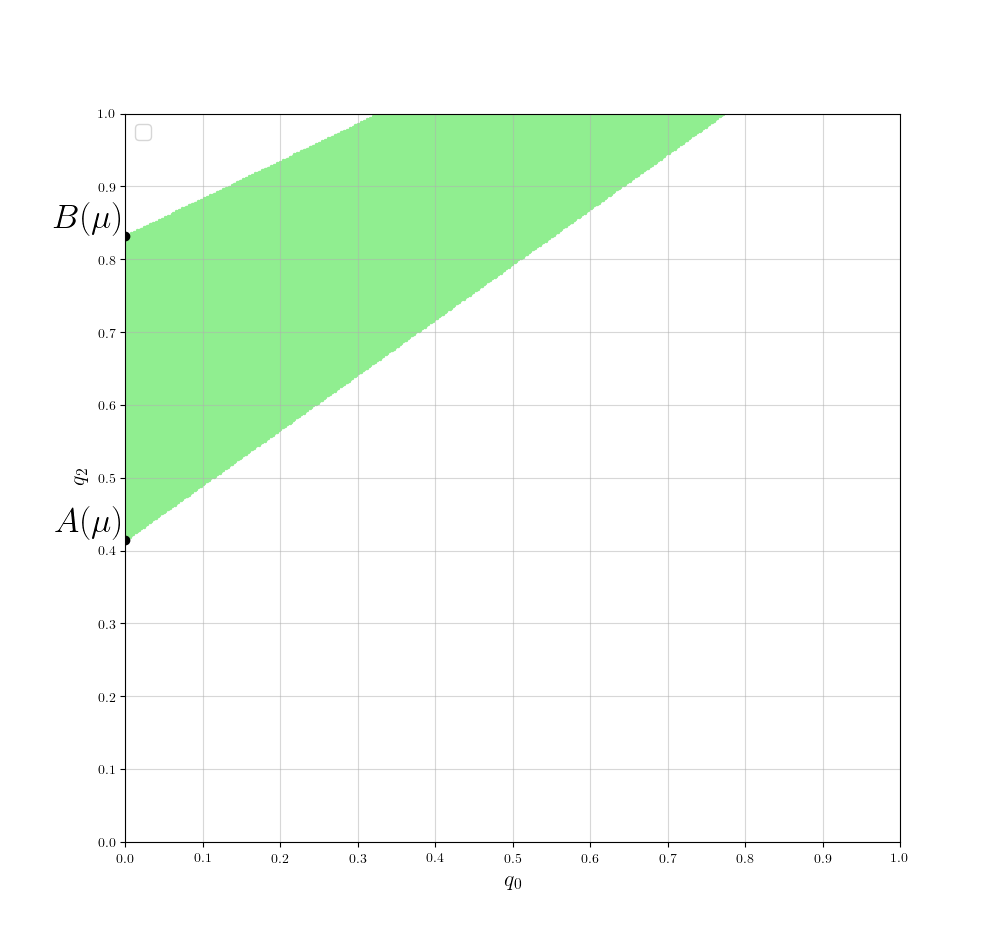
\includegraphics[width=\linewidth]{part_2/graf_3_7}
		\caption{
			$\mu \in (0, 1), 
			\lambda \in (2\frac{1 - \mu}{2 - \mu}, 1]$		
		}
	\end{subfigure}
	\begin{subfigure}[b]{0.3 \textwidth}
		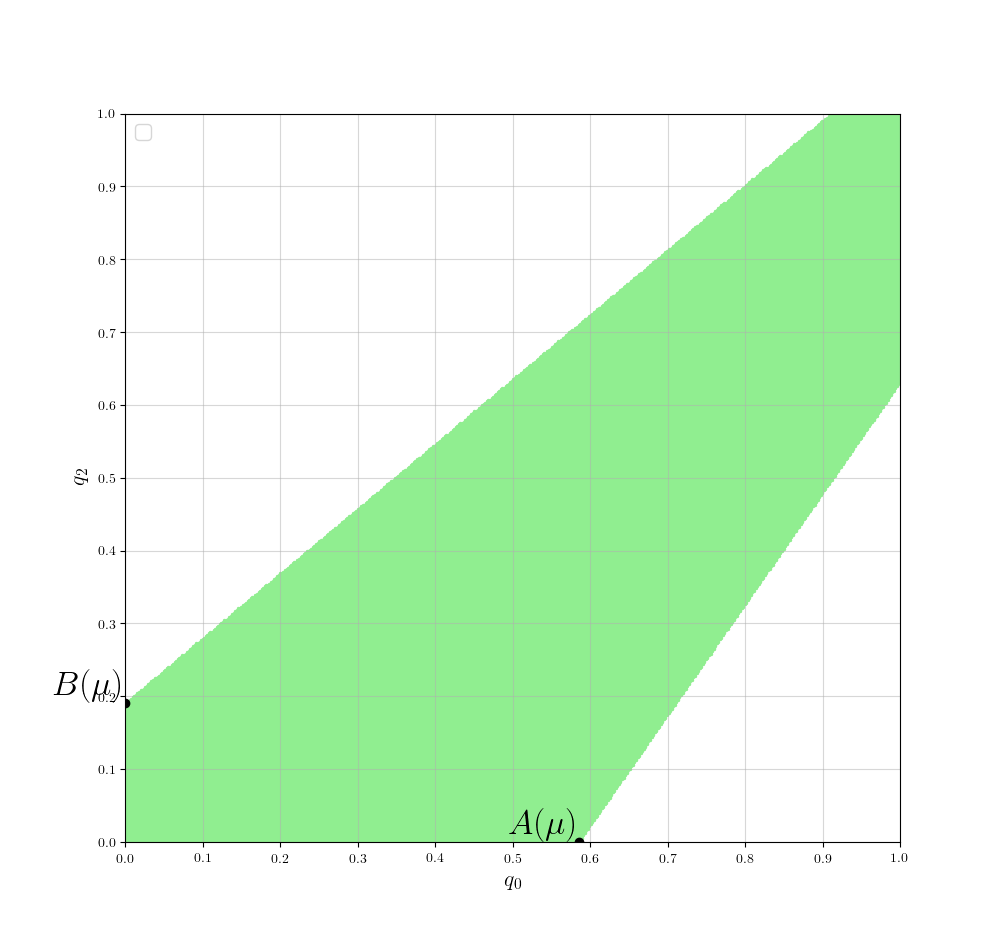
\includegraphics[width=\linewidth]{part_2/graf_3_8}
		\caption{
			$\mu = 1, \lambda \in (0, 1] $		
		}
	\end{subfigure}
	\caption{}
\end{figure}
%\section{Графическое изображение матожидания критерия}
Вычислим матожидание от имеющегося векторного критерия для игрока П
$F(X, Y) = \big(\frac{Y\sqrt{X}}{2};\frac{\sqrt{1-X}}{Y}\big)$, где $X$ и $Y$ - случайные величины, причём
\[
\begin{cases}
P(X=0)=1-q \\
P(X=1)=q \\
\end{cases}
\begin{cases}
P(Y=1)=1-p \\
P(Y=2)=p \\
\end{cases}
\]

В таком случае имеем:
\begin{equation}
\E_{x} [F(x,y)]=\big(\frac{yq}{2};\frac{1-q}{y}\big)
\end{equation}
\begin{equation}
\E_{xy} [F(x,y)]=\big(\frac{q(1+p)}{2};\frac{(1-q)(2-p)}{2}\big)
\end{equation}

Рассмотрим это как множество точек на плоскости $X,Y$ зависящие от двух параметров $(p,q)\in[0,1]^2$
\[
\begin{cases}
y=\frac{q(1+p)}{2} \\
x=\frac{(1-q)(2-p)}{2}  
\end{cases}
\Rightarrow
\begin{cases}
q=\frac{2x}{1+p} \\
y=(1-\frac{2x}{1+p})\frac{2-p}{2}=\frac{(1+p-2x)(2-p)}{2(1+p)}
\end{cases}
\]

Найдём максимальные значения, которые может принимать $y(x, p)$ при фиксированном $x$:
$$
\frac{\partial{y(x,p)}}{\partial{p}}=\frac{3x}{(p+1)^2} - \frac{1}{2}=0 
\Rightarrow
p_0=\sqrt{6x} - 1
$$
Поскольку область определения $p_0\in[0, 1]$, и 
$$
p_0 = 1 \Rightarrow x=\frac{2}{3} \textsl{ и }
p_0 = 0 \Rightarrow x=\frac{1}{6}
$$
 
$$y_{max}(x) = 
\begin{cases}
\max(y(x, 0), y(x, 1), y(x, p_0)), & x\in[\frac{1}{6}, \frac{2}{3}] \\
\max(y(x, 0), y(x, 1)), & x\in[0, \frac{1}{6}] \cap [\frac{2}{3}, 1]
\end{cases}
$$

учитывая, что 
$$y(x, 0) = 1 - 2x $$
$$y(x, 1) = \frac{1-x}{2}$$ 
$$y(x,p_0) = \frac{(\sqrt{6x} - 2x)(3-\sqrt{6x})}{2\sqrt{6x}}$$

$$y_{min}(x)=
\begin{cases}
\frac{1-x}{2}, &x\in[0,\frac{1}{3}] \\
1-2x, &x\in(\frac{1}{3},1]
\end{cases}
\quad
y_{max}(x)=
\begin{cases}
1-2x, &x\in[0,\frac{1}{6}] \\
\frac{(\sqrt{6x} - 2x)(3-\sqrt{6x})}{2\sqrt{6x}}, &x\in(\frac{1}{6},\frac{2}{3}]\\
\frac{1-x}{2}, &x\in(\frac{2}{3},1]
\end{cases}
$$

В предыдущем пункте мы установили что любая пара $(p^{*}, q^{*}) \in [0, 1]^{2}$ является оптимальной. Теперь для всех
оптимальных стратегий т.е. пар $(p^{*}, q^{*}) \in [0, 1]^{2}$ изобразим на графике значения матожидания векторного критерия в этой
точке.
\begin{center}
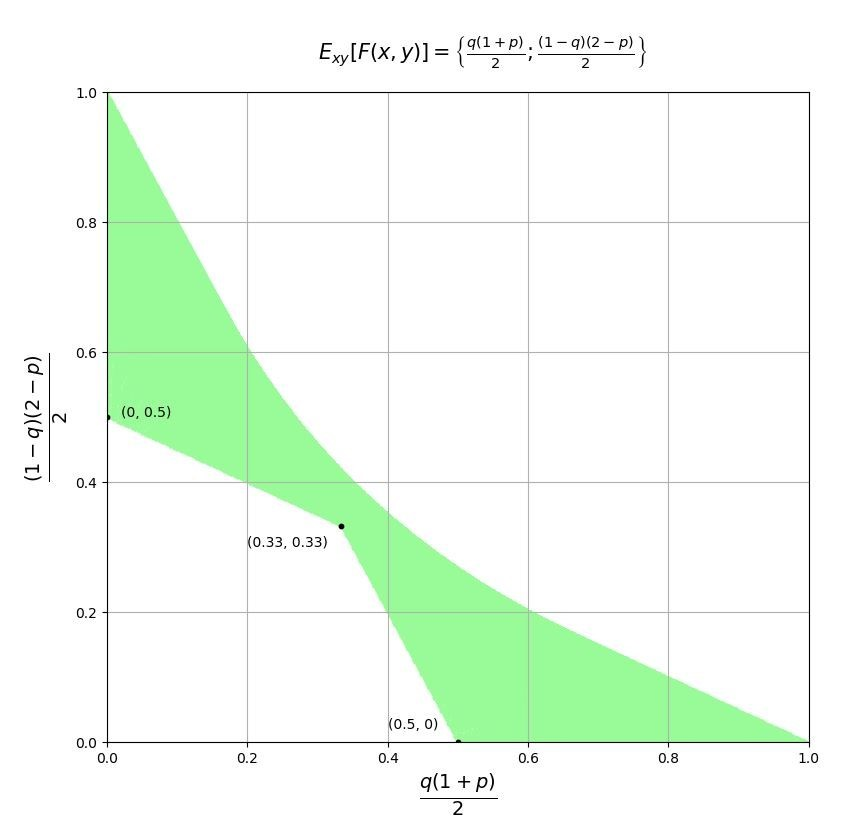
\includegraphics[scale=0.8]{part_2/graf_1_2}
\end{center}


%\section{Выигрыш игрока Студент}

Теперь на квадрате $(\mu, \lambda) \in [0, 1]^2$ мы рассмотрели все точки
и для каждой нашли оптимальные пары $p^*(\mu, \lambda)$
и $q^*(\mu, \lambda)$ и соответсвующие значения функции 
$M(p^*(\mu, \lambda),q^*(\mu, \lambda),\mu)$. Далее на квадрате
$[0, 1]^{2}$ изобразим все точки, которые принимает вектор $(\mu M(p^*,q^*,\mu), (1-\mu) M(p^*,q^*,\mu))$ при
$(\mu, \lambda)\in[0, 1]^{2}$

\begin{center}
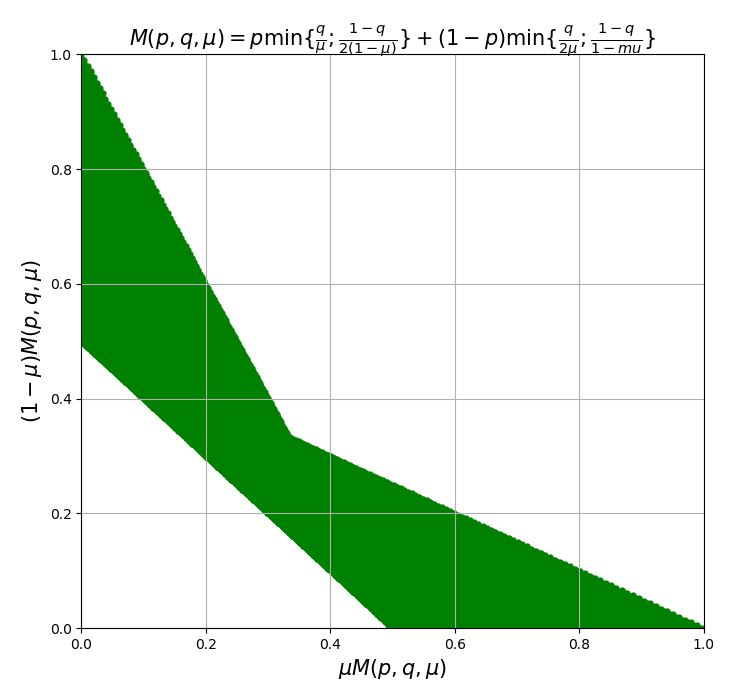
\includegraphics[scale=0.6]{part_2/graf_4}
\end{center}

Поясним график: \\
нижняя огибающая в координатах $X,Y$: $y=\dfrac{1}{2}-x$, \\
верхняя огибающая в координатах $X,Y$: 
$y=
\begin{cases}
	1 - 2x, & x \in [0, \dfrac{1}{3}) \\
	\dfrac{1 - x}{2}, & x \in [\dfrac{1}{3}, 1]
\end{cases}.
$

И найдём множества значений функции 

$$
	\overline G(p, q, \mu)=
	p \min \{
		\dfrac{q}{\mu};
		\dfrac{1-q}{2(1-\mu)}
	\} + (1 - p) \min \{
		\dfrac{q}{2\mu};
		\dfrac{1 - q}{1 - \mu}
	\},
$$

В этих областях
Далее рассмотрим игру с точки зрения игрока С. 
найдём значение свёртки для игрока С в этих точка:

, тогда

$
	\overline G(1, 0, 0) = \dfrac{1}{2}
$

$
	\overline G([0, 1], 0, 0) = [0.5, 1]
$

$	
	\overline G([0, 1], 1, 1) = [0.5, 1]
$

$
	\overline G(1, \dfrac{\mu}{2 - \mu}, \mu)=
	\min \big\{
		\dfrac{\mu}{2 - \mu}; 
		\dfrac{1 - \dfrac{\mu}{2 - \mu}}{2(1 - \mu)}
	\big\}
	=\dfrac{1}{2 - \mu}
$

$
	\overline G(1,\dfrac{\mu}{2-\mu},\mu)=\dfrac{1}{2-\mu}
$

$
	\overline G(p,\dfrac{2\mu}{1+\mu},\mu) =
	p\dfrac{1}{2(1 + \mu)} + (1 - p)\dfrac{1}{1 + \mu}=
	\dfrac{2 - p}{2(1 + \mu)} \geqslant
	\dfrac{2 - (1 - \mu)}{2(1 + \mu)} =
	\dfrac{1 + \mu}{2(1 + \mu)} =
	\dfrac{1}{2}
$

$
	\overline G(p, \dfrac{2\mu}{1 + \mu}, \mu) \leqslant 
	\dfrac{1}{1 + \mu} \Rightarrow
	\overline G (p, \dfrac{2\mu}{1 + \mu}, \mu) = 
	[0.5, 	\dfrac{1}{1 + \mu}]
$

$
	\overline G(0, \dfrac{2\mu}{1 + \mu}, \mu) = 
	\dfrac{1}{1 + \mu}
$

$
	\overline G(1, \dfrac{\mu}{2 - \mu}, \mu) = 
	\dfrac{1}{2 - \mu}
$

$
	\overline G(0, \dfrac{2\mu}{1 + \mu}, \mu) = 
	\dfrac{1}{1 + \mu}
$

$
	\overline G(p, \dfrac{\mu}{2 - \mu}, \mu) =
	p\dfrac{1}{2 - \mu} + (1 - p)\dfrac{1}{2(2 - \mu)} =
	\dfrac{1 + p}{2(2 - \mu)} \geqslant 
	\dfrac{2 - \mu}{2(2 - \mu)} =
	\dfrac{1}{2}
$

$
	\overline G(p, \dfrac{\mu}{2 - \mu}, \mu) \leqslant
 	\dfrac{1}{2 - \mu} \Rightarrow 
 	\overline G(p, \dfrac{\mu}{2 - \mu}, \mu) =
 	[0.5, \dfrac{1}{2 - \mu}]
$

$
	\overline G(0, \dfrac{2\mu}{1 + \mu}, \mu)=
	\min \big\{
		\dfrac{1}{\mu}\dfrac{2\mu}{1 + \mu}; 
		\dfrac{1 - \dfrac{2\mu}{1 + \mu}}{1 - \mu}
	\big\} =
	\dfrac{1}{1 + \mu}
$

$
	\overline G(0, 1, 1) = \dfrac{1}{2}
$

%\section{Постановка задача}

\begin{flushleft}

	Функциональный критерий: 
	$F(x, y) = (\frac{y\sqrt{x}}{2},\frac{\sqrt{1-x}}{y})$
	

	
	\begin{center}
	\begin{tabu} to 0.8 \textwidth {X[c] X[c]}
		$\textrm{С:  }F(x, y) \rightarrow \max \limits_{x\in X}$	&
		$\textrm{П:  }F(x, y) \rightarrow \min \limits_{y \in Y}$ \\
		$X = \{ 0; \frac{1}{2}; 1\}$ & $Y = \{1, 2\}$	\\
		\\
		$P(X=0)=q_0$ & $P(Y=1)=p_0$ \\
		$P(X=\frac{1}{2})=q_1$ & $P(Y=2)=p_1$ \\
		$P(X=1)=q_2$ & 
		\\
		$\sum \limits_{i=0}^2 q_i=1$ & $\sum \limits_{i=0}^1 p_i=1$ \\
		$0 \leqslant q_i \leqslant 1 \;,\;\; i=\overline{0,2}$ &
		$0 \leqslant p_i \leqslant 1 \;,\;\; i=\overline{0,1}$  \\
		\\
		$\textrm{Следровательно  } q_1 = 1-q_0-q_2$ & 
		$\textrm{Пусть  } p := p_1, \textrm{ тогда }\; p_0=1-p$ 
	\end{tabu}	
	\end{center}

	Введём множество 
	\begin{equation}
		Q=\{(q_0,q_2) \in \mathbb{R}^2 \; | \;
		0 \leqslant q_i \leqslant 1 \; i\in\{0,2\}; \; 
		q_0 + q_2 \leqslant 1\}	
	\end{equation}


	Студент выбирет $X$ и использует \textbf{ОЛС}. \\
	Преподаватель выбирает $Y$ и использует \textbf{ЛС}.\\
\end{flushleft}
%\section{Оптимальные значения}

\subsection{Рассмотрим игру за преподавателя}
\begin{flushleft}
	Игрок использует смешанную стратегию:\\
	
	$$
	F_\textrm{П}(p,x)=
	\big \langle 
		(1-p)\frac{1 \cdot \sqrt{x}}{2} + p \frac{2 \cdot \sqrt{x}}{2}; \;
		(1-p)\frac{\sqrt{1-x}}{1}+p\frac{\sqrt{1-x}}{2} 
	\big \rangle=
	\frac{1}{2}
	\big \langle
		(p+1)\sqrt{x}; \;
		(2-p)\sqrt{1-x}
	\big \rangle
	$$
	
	Игрок использует ЛС:
	
	$$
	L(p,x,\lambda)=
	\frac{1}{2}
	\big(
		\lambda(p+1)\sqrt{x} + (1-\lambda)(2-p)\sqrt{1-x}
	\big)
	$$
	
	Введём обозначение $q=(q_0,q_1,q_2)$ и осредняем по переменной $x$:
	
	$$ 
	\overline{L}(p,q,\lambda)=
	\frac{1}{2} 
	\Big(
		q_0(1-\lambda)(2-p)\sqrt{1}+
		q_1 \big (\lambda(p+1)\frac{1}{\sqrt{2}} + 
		(1-\lambda)(2-p)\frac{1}{\sqrt{2}} \big )+
		q_2\lambda(p+1)\sqrt{1}
	\Big)=
	$$
	$$
	=\frac{1}{2\sqrt{2}}
	\Big (
		\big (\lambda(q_1+\sqrt{2}q_2)-(1-\lambda)(q_1+\sqrt{2}q_0) \big)p+
		\big (\lambda(q_1+\sqrt{2}q_2)+2(1-\lambda)(q_1+\sqrt{2}q_0) \big)
	\Big)
	$$
	Итого получаем:
	$$
	\overline{L}(p,q,\lambda)=k(\lambda,q)p+b(\lambda,q)
	$$
	где
	$$
	k(q, \lambda) = \frac{1}{2\sqrt{2}}
		\big (\lambda(q_1+\sqrt{2}q_2)-(1-\lambda)(q_1+\sqrt{2}q_0) \big)
	$$
	$$
	b(q, \lambda) = \frac{1}{2\sqrt{2}}
		\big (\lambda(q_1+\sqrt{2}q_2)+2(1-\lambda)(q_1+\sqrt{2}q_0) \big)
	$$
	
	Наша задача найти 
	$\hat p(q, \lambda)=\arg \min \limits_{p \in [0, 1]} \overline{L}(p,q,\lambda)$.
	Поскольку функция $\overline{L}(p,q,\lambda)$ линейна по переменной 
	$p$, следовательно:
	
	$$
		\hat p(q, \lambda)=
		\arg \min \limits_{p \in [0, 1]} \overline{L}(p,q,\lambda)=
		\begin{cases}
			0, & k(\lambda,q)>0 \\
			1, & k(\lambda,q)<0 \\
			[0,1], & k(\lambda,q)=0
		\end{cases}	
	$$
	
	Рассмотрим функцию $k(q, \lambda)=\frac{1}{2\sqrt{2}}
	\Big(
		\lambda \big (2+(\sqrt{2}-2)(q_0-q_2) \big) -
		\big (1 - q_2 + (\sqrt{2} - 1)q_0 \big)
	\Big)
	$

	Введём обозначения:
	
	$$\ell(q) = \frac{1 - q_2 + (\sqrt{2} - 1)q_0}{2+(\sqrt{2}-2)(q_0-q_2)}$$	
	
	Поскольку для $q$ удовлетворяющих заданным ограничениям	верно: 
	$$2+(\sqrt{2}-2)(q_0-q_2) > 0$$
	
	Следовательно:
	
	$$
	k(q, \lambda) \vee 0 \Leftrightarrow 
	\lambda \vee \ell(q)
	$$
	
	На рисунке 1 в плоскости $q=(q_0.q_2)$ бирюзовым 
	цветом изображена область в которой $0 \leqslant \ell(q) \leqslant 1$.
	Видно, что квадрат $q = [0,1]^2$ полностью принадлежит этой области.
	Прямые $\ell_1(q)$ и $\ell_2(q)$ такие, что:
	$$\ell_1(q): \; \ell(q)=0 $$
	$$\ell_2(q): \; \ell(q)=1 $$
	
	\begin{figure}[H]
		\centering
  		\includegraphics[scale=0.5]{images/graf_3_1}
  		\caption{}
	\end{figure}
	
	Следовательно $\forall q=(q_0, q_2) \in [0,1]^2 \;
	\exists \; \lambda \in [0,1]: \; k(\lambda,q)=0$  
	
	$$
		\hat p(\lambda,q)=
		\arg \min \limits_{p \in [0, 1]} \overline{L}(p,q,\lambda)=
		\begin{cases}
			0, & \lambda \in \big(\ell (q), 1\big] \\
			1, & \lambda \in \big[0, \ell(q) \big) \\
			[0,1], & \lambda=\ell(q)
		\end{cases}
		\textrm{ , где } \ell(q)=
		\frac{1 - q_2 + (\sqrt{2} - 1)q_0}{2+(\sqrt{2}-2)(q_0-q_2)}
	$$	
	
\end{flushleft}
%\subsection{Рассмотрим игру за студента}
\begin{flushleft}

	Игрок \textbf{С} стремится максимизировать функциональный критерий: 
	
	$$F(x, y) = (\frac{y\sqrt{x}}{2},\frac{\sqrt{1-x}}{y})$$	

	Игрок \textbf{С} использует смешанную стратегию, т.е. его стратегией является
	распределение $q=(q_0,q_1,q_2)$ над множеством чистых стратегий 
	$X=\{0,\frac{1}{2},1\}$:\\

	$$
		F_\textrm{C}=
		\big \langle
			q_0\frac{y\sqrt{0}}{2} + 
			q_1\frac{y}{2} \sqrt{\frac{1}{2}} + 
			q_2\frac{y\sqrt{1}}{2};
			q_0\frac{\sqrt{1}}{y} +
			q_1\frac{1}{y} \sqrt{\frac{1}{2}} +
			q_2\frac{\sqrt{0}}{y}
		\big \rangle = 
	$$
	$$
		=\big \langle
			\frac{y}{2}\cdot\frac{1-q_0+(\sqrt{2}-1)q_2}{\sqrt{2}};
			\frac{1}{y}\cdot\frac{1-q_2+(\sqrt{2}-1)q_0}{\sqrt{2}}
		\big \rangle
	$$	
	
	Затем использует \textbf{ОЛС} (2). Сначала рассмотрим вырожденные случаи \\
	когда $\mu=0$ и  $\mu=1$. 

%-----------------------------------------------------------------------

	\textbf{(1)} Если $\mu=0$:
	$$
		G(y,q,0)=\frac{1}{\sqrt{2}}\cdot \frac{1-q_2+(\sqrt{2}-1)q_0}{y}
	$$	
	
	Далеем осредняем функцию $G(y,q,\mu)$ по стратегиям 
	противника $y \in Y=\{1,2\}$ c вероятностями $(1-p,p)$:
	\begin{gather*}
		\overline G(p,q,0)=
		\frac{1-p}{\sqrt{2}} \cdot \frac{1-q_2+(\sqrt{2}-1)q_0}{1}+
		\frac{p}{\sqrt{2}} \cdot \frac{1-q_2+(\sqrt{2}-1)q_0}{2}=\\
		=\frac{(2-p)(1-q_2+(\sqrt{2}-1)q_0)}{2\sqrt{2}}
	\end{gather*}
	
	Найдём частные производную по переменным $q_0$ и $q_2$, при этом
	введём следующие обозначения для сокращения записи:
	
	\begin{equation}\label{eq:G_dericative}
		\frac{\partial \overline G(p,q,\mu)}{\partial q}
		=\langle \frac{\partial \overline G(p,q,\mu)}{\partial q_0};
		\frac{\partial \overline G(p,q,\mu)}{\partial q_2} \rangle=
		\langle g_1(p,q,\mu), g_2(p,q,\mu) \rangle
	\end{equation}

	$$
		\frac{\partial \overline G(p,q,0)}{\partial q}
		=\frac{2-p}{2\sqrt{2}} \langle \sqrt{2}-1;-1\rangle
	$$
	Поскольку $p \leqslant 1$, то $\dfrac{2-p}{2\sqrt{2}} > 0 $.
	Мы рассматриваем задачу максимизации \\ на множестве $(3)$.
	Следовательно:
	$$q^* = \arg \max \limits_{q \in Q} \overline G(p,q,0)=(1,0).$$

%--------------------------------------------------------------------
	
	\textbf{(2)} Если $\mu=1:$
	$$
		G(y,q,1)=\frac{1}{\sqrt{2}}\cdot \frac{1-q_2+(\sqrt{2}-1)q_0}{y}
	$$	
	
	Далеем осредняем функцию $G(y,q,\mu)$ по стратегиям 
	противника $y \in Y=\{1,2\}$ c вероятностями $(1-p,p)$:
	
	\begin{gather*}
		\overline G(p,q,1)=
		\frac{1-p}{\sqrt{2}} \cdot \frac{1-q_0+(\sqrt{2}-1)q_2}{2}+
		\frac{p}{\sqrt{2}} \cdot \frac{1-q_0+(\sqrt{2}-1)q_2}{1}=\\
		=\frac{(p+1)(1-q_0+(\sqrt{2}-1)q_2)}{2\sqrt{2}}
	\end{gather*}
	
	Найдём частные производную по переменным $q_0$ и $q_2$:	
	
	$$
		\frac{\partial \overline G(p,q,1)}{\partial q}
		=\frac{p+1}{2\sqrt{2}} \langle -1; \sqrt{2}-1\rangle
	$$
	
	Поскольку $p \geqslant 0$, то $\dfrac{p+1}{2\sqrt{2}} > 0 $.
	Мы рассматриваем задачу максимизации \\ на множестве $(3)$.
	Следовательно:
	$$q^* = \arg \max \limits_{q\in Q} \overline G(p,q,1)=(0,1).$$

%--------------------------------------------------------------------
		
	\textbf{(3)} Теперь $\mu \neq 0,1$:
	$$
		G(y,q,\mu)=\frac{1}{\sqrt{2}}\min \limits_{0<\mu<1}
		\big \langle
			\frac{y}{2} \cdot \frac{1-q_0+(\sqrt{2}-1)q_2}{\mu};
			\frac{1}{y} \cdot \frac{1-q_2+(\sqrt{2}-1)q_0}{1-\mu}
		\big \rangle	
	$$

	Далеем осредняем функцию $G(y,q,\mu)$ по стратегиям 
	противника $y \in Y=\{1,2\}$ c вероятностями $(1-p,p)$:

	\begin{multline}\label{eq:G_aver}
		\overline G(p,q,\mu)=\frac{1-p}{\sqrt{2}}\min \limits_{0<\mu<1}
		\big \langle
			\frac{1-q_0+(\sqrt{2}-1)q_2}{2\mu};
			\frac{1-q_2+(\sqrt{2}-1)q_0}{1-\mu}
		\big \rangle + \\
		+\frac{p}{\sqrt{2}}\min \limits_{0<\mu<1}
		\big \langle
			\frac{1-q_0+(\sqrt{2}-1)q_2}{\mu};
			\frac{1-q_2+(\sqrt{2}-1)q_0}{2(1-\mu)}
		\big \rangle 
	\end{multline}
	
	Введём вспомогательные обозначения:
	
	\begin{gather*}
		\ell_1(q,\mu)=\frac{1-q_0+(\sqrt{2}-1)q_2}{2\mu} \\
		\ell_2(q,\mu)=\frac{1-q_2+(\sqrt{2}-1)q_0}{1-\mu} \\
		\ell_3(q,\mu)=\frac{1-q_0+(\sqrt{2}-1)q_2}{\mu} \\
		\ell_4(q,\mu)=\frac{1-q_2+(\sqrt{2}-1)q_0}{2(1-\mu)}
	\end{gather*}
	
	
	Для различных значений переменной $\mu$ рассмотрим 
	взаимные расположения множеств $\ell_1>\ell_2$ и $\ell_3>\ell_4$
	на плоскости $(q_0,q_2)$. Другими словами для фиксированного 
	значения $\mu \in [0,1]$ найдём области плоскости, в которых 
	достигается минимум одного из выражений в (5):
	
	\begin{figure}[H]
    	\centering
     	\begin{subfigure}[b]{0.22 \textwidth}
        	\centering
        	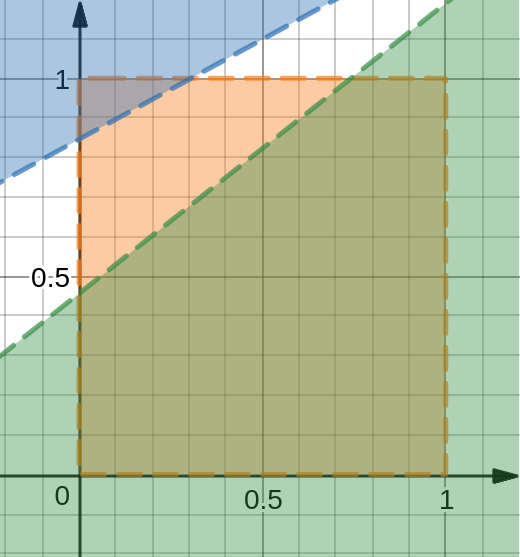
\includegraphics[width=\textwidth]{images/graf_6_1}
        	\caption{$\mu=0.8$}
         	\label{fig:y equals x}
     	\end{subfigure}
     	\hfill
     	\begin{subfigure}[b]{0.22 \textwidth}
        	\centering
        	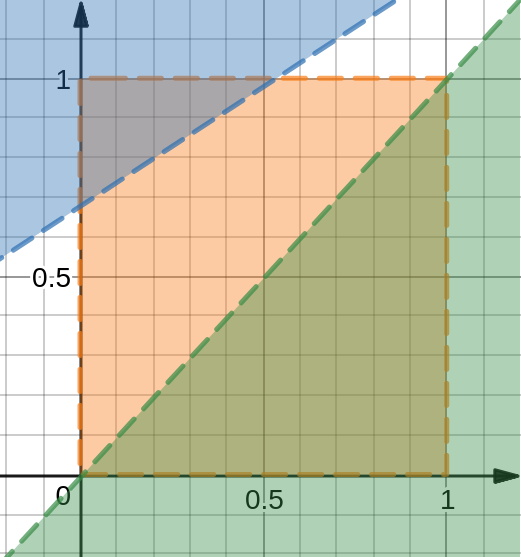
\includegraphics[width=\textwidth]{images/graf_6_2}
        	\caption{$\mu=\frac{2}{3}$}
        	\label{fig:three sin x}
     	\end{subfigure}
     	\hfill
     	\begin{subfigure}[b]{0.22 \textwidth}
        	\centering
        	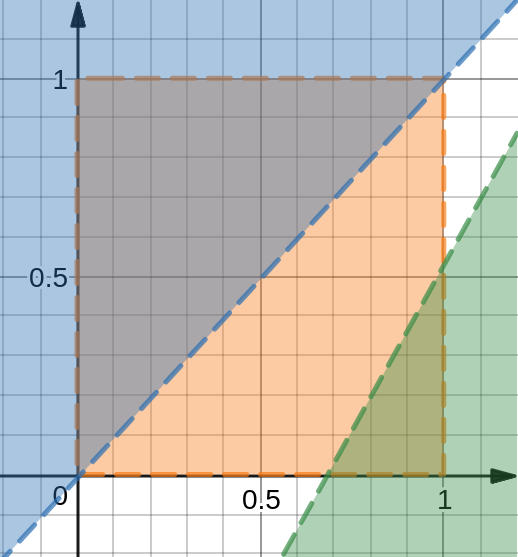
\includegraphics[width=\textwidth]{images/graf_6_3}
        	\caption{$\mu=\frac{1}{3}$}
        	\label{fig:five over x}
     	\end{subfigure}
     	\hfill
     	\begin{subfigure}[b]{0.22 \textwidth}
        	\centering
        	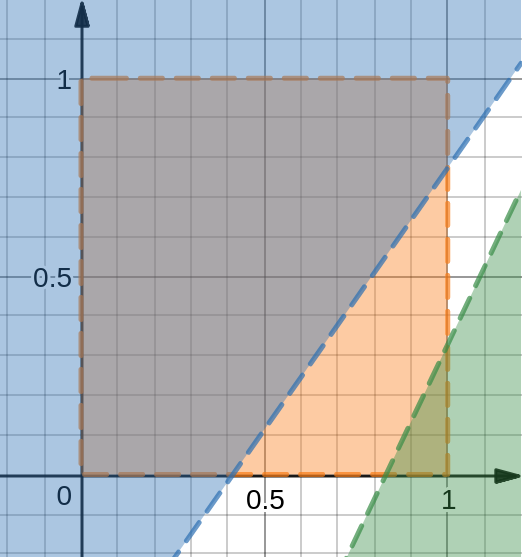
\includegraphics[width=\textwidth]{images/graf_6_4}
         	\caption{$\mu=0.1$}
         	\label{fig:five over x}
     	\end{subfigure}
	\end{figure}
	
	Поясним график. Синяя область - это множество $\ell_1 > \ell_2$.\\
	Зелёная область на графике - это множнство $\ell_3 < \ell_4$.\\
	Область между ними - это множество $\{\ell_1<\ell_2 \cap \ell_3 > \ell_4\}$.
	Исходя из графиков $\{\ell_1>\ell_2 \cap \ell_3 < \ell_4\} = \emptyset$ 
	при $(\mu, q) \in (0, 1) \times [0, 1]^2$.
	Поскольку граничные случаи для параметра $\mu$ были рассмотрены в первых
	двух пунктах, то квадрат $[0,1]^2$ на плоскости $(q_0,q_2)$ делится на 3 не 
	пересекающихся множества.
	
	\textbf{Добавить доказательство того, что всего три возможных варианта}

	\textbf{(1)} Рассмотрим полуплоскость, которая определяется системой
	$\begin{cases}
			\ell_1 > \ell_2 \\
			\ell_3 > \ell_4
	\end{cases} \sim \; \l_1 > l_2$
	
	Выражение \eqref{eq:G_aver} на этом множестве принимает следующий вид:
	
	\begin{gather*}
		\overline G(p,q,\mu)=
		\frac{1-p}{\sqrt{2}} \cdot \frac{1-q_2+(\sqrt{2}-1)q_0}{1-\mu} + 
		\frac{p}{\sqrt{2}} \cdot \frac{1-q_2+(\sqrt{2}-1)q_0}{2(1-\mu)} = \\
		=\frac{2-p}{2\sqrt{2}}\cdot\frac{1-q_2+(\sqrt{2}-1)q_0}{1-\mu}		
	\end{gather*}
	
	\textbf{(2)} Рассмотрим полуплоскость, которая определяется системой
	$\begin{cases}
			\ell_1 < \ell_2 \\
			\ell_3 < \ell_4
	\end{cases} \sim \; \l_3 < l_4$
	
	Выражение \eqref{eq:G_aver} на этом множестве принимает следующий вид:
	
	\begin{gather*}
		\overline G(p,q,\mu)=
		\frac{1-p}{\sqrt{2}} \cdot \frac{1-q_0+(\sqrt{2}-1)q_2}{2\mu} + 
		\frac{p}{\sqrt{2}} \cdot \frac{1-q_0+(\sqrt{2}-1)q_2}{\mu} = \\
		=\frac{1+p}{2\sqrt{2}}\cdot\frac{1-q_0+(\sqrt{2}-1)q_2}{\mu}		
	\end{gather*}
	
	\textbf{(3)} Рассмотрим область, которая определяется системой
	$\begin{cases}
			\ell_1 < \ell_2 \\
			\ell_3 > \ell_4
	\end{cases}$

	Выражение \eqref{eq:G_aver} на этом множестве принимает следующий вид:	
	
	\begin{gather*}	
		\overline G(p,q,\mu)=
		\frac{1-p}{\sqrt{2}} \cdot \frac{1-q_0+(\sqrt{2}-1)q_2}{2\mu} +
		\frac{p}{\sqrt{2}} \cdot \frac{1-q_2+(\sqrt{2}-1)q_0}{2(1-\mu)}=\\	
		=\frac{(1-p)(1-\mu)(1-q_0+(\sqrt{2}-1)q_2)+p\mu(1-q_2+(\sqrt{2}-1)q_0)}
		{2\sqrt{2}\mu(1-\mu)}
	\end{gather*}
	
	Итого: 
	
	$$
	\overline G(p,q,\mu) =		
	\begin{cases}
		\dfrac{2-p}{2\sqrt{2}}\cdot\dfrac{1-q_2+(\sqrt{2}-1)q_0}{1-\mu} 
		,\hspace{2mm} \ell_1 \geqslant \ell_2		
		\\
		\dfrac{1+p}{2\sqrt{2}}\cdot\dfrac{1-q_0+(\sqrt{2}-1)q_2}{\mu}
		,\hspace{2mm} \ell_3 \leqslant \ell_4\\
		\dfrac{(1-p)(1-\mu)(1-q_0+(\sqrt{2}-1)q_2)+p\mu(1-q_2+(\sqrt{2}-1)q_0)}
		{2\sqrt{2}\mu(1-\mu)}
		,\hspace{2mm}
		\begin{cases}
			\ell_1 \leqslant \ell_2\\
			\ell_3 \geqslant \ell_4\\
		\end{cases}
	\end{cases}
	$$	
	
	Тогда производная от функции имеет:
	
	$$
	\frac{\partial \overline{G}(p,q,\mu)}{\partial q}=
	\begin{cases}
		\dfrac{2-p}{2\sqrt{2}(1-\mu)} \langle \sqrt{2}-1; -1 \rangle 
 		,\hspace{2mm}
 		\ell_1 \geqslant \ell_2\\
		
		\dfrac{1+p}{2\sqrt{2}\mu} \langle -1; \sqrt{2}-1 \rangle
		,\hspace{2mm}
		\ell_3 \leqslant \ell_4\\
		
		\dfrac{1}{2\sqrt{2}\mu(1-\mu)}
		\big \langle 
			(\sqrt{2} - 1)p\mu -(1-p)(1-\mu);
			(\sqrt{2} - 1)(1-p)(1-\mu) - p\mu			
		\big \rangle
		,\hspace{2mm}
		\begin{cases}
			\ell_1 \leqslant \ell_2\\
			\ell_3 \geqslant \ell_4\\
		\end{cases}
	\end{cases}
	$$
	
%------------------------------------------------------------

	\textbf{(1)} Рассмотрим $\ell_1 \geqslant \ell_2$. 
	Производная в области имеет вид:
	
	$$\frac{\partial \overline{G}(p,q,\mu)}{\partial q}=
	\frac{2-p}{2\sqrt{2}(1-\mu)} \langle \sqrt{2}-1; -1 \rangle$$
 	
	Введём вспомогалетльную функцию	
 	$\ell_B(q, \mu):=(\ell_1-\ell_2) \cdot \mu(1-\mu)$,
 	множество, на котором она принимает неотрицательные значения 
 	составляют интересующую нас область. Множитель $\mu(1-\mu)$ является строго
 	положительным на $\mu \in (0,1)$, поэтому не влияет на знак. Функция
 	является линейной по переменным $q_0$ и $q_2$:
 	
	$$\ell_B(q, \mu) = 
	(1+\mu(2\sqrt{2}-3))q_0+
	(1-\sqrt{2}+\mu(\sqrt{2}-3))q_2
	+3\mu-1$$ 	
	
	Параметр $\mu$ изменяется в диапазоне $(0,1)$, причём	
	
	\begin{gather*}	
	\ell_B(q,\mu) \xrightarrow[\mu\rightarrow 1]{} 
	1-q_0+(\sqrt{2}-1)q_2\\	
	\ell_B(q,\mu) \xrightarrow[\mu\rightarrow 0]{} 	
	1-q_2+(\sqrt{2}-1)q_0\\
	\end{gather*}
	
	Предельные положения $\ell_B(q, \mu)=0$ изображены на графике \eqref{fig:l_B_limits}.
	
	\begin{figure}[H]
		\centering
  		\includegraphics[scale=0.3]{images/graf_3_2}
  		\caption{}
  		\label{fig:l_B_limits}
	\end{figure}	
	
	Найдём значение $\mu$ при котором прямая $\ell_B(q, \mu)$ проходит через точку
	$q=(0,0)$:
	
	$$\ell_B(0,0,\hat \mu) = 0
	\Rightarrow \hat \mu = \frac{1}{3}$$	
	
	Очевидно, что на полиэдре $P_B(\mu):$
		
	$$P_B(\mu)=\{q \in Q \; | 
	\;  \ell_B(q, \mu) \geqslant 0 \}, \; \mu \in (0,1)$$
	
	функция $\overline{G}(p,q,\mu)$ достигает максимума в точке $B(\mu):$
	
	$$
	q^* = \arg \max \limits_{q\in P_B(\mu)} \overline G(y,q,\mu) = B(\mu)=
	\begin{cases}
		(0, q_2) : \ell_B(0,q_2,\mu)=0, & \frac{1}{3} \leqslant \mu < 1 \\
		(q_0, 0) : \ell_B(q_0,0,\mu)=0, & 0 < \mu \leqslant \frac{1}{3} \\
	\end{cases}	
	$$
	
	\begin{figure}[H]
    	\centering
     	\begin{subfigure}[b]{0.4 \textwidth}
        	\centering
        	\includegraphics[width=\textwidth]{images/graf_3_3}
        	\caption{$\mu=0.1 < \frac{1}{3}$}
         	\label{fig:y equals x}
     	\end{subfigure}
     	\hspace{10mm}
     	\begin{subfigure}[b]{0.4 \textwidth}
        	\centering
        	\includegraphics[width=\textwidth]{images/graf_3_4}
        	\caption{$\mu=0.4 > \frac{1}{3}$}
        	\label{fig:three sin x}
     	\end{subfigure}
	\end{figure}	

	На графике зелёным цветом изображена область $P_B(\mu)$, чёрным цветом
	обозначены линии уровня и стрелкой соответсвенно градиент функции.
	Рассмотрим эти два случая и найдём явное выражение для точки $B(\mu)$:
	
	\textbf{(a)} Если $\frac{1}{3} \leqslant \mu \leqslant 1$ то координата $q_2$ точки 
	максимума определяется из условия: 
	
	\begin{gather*}
		\ell_B(0,q_2,\mu)=0
		\\
		(1-\sqrt{2}+\mu(\sqrt{2}-3))q_2+3\mu-1=0
		\hspace{3mm} \Rightarrow \hspace{3mm}
		q_2=\frac{3\mu-1}{\sqrt{2}-1+(3-\sqrt{2})\mu}	
		\\
		q^*=(0;\dfrac{3\mu-1}{\sqrt{2}-1+(3-\sqrt{2})\mu}), \hspace{3mm}
		\frac{1}{3} \leqslant \mu \leqslant 1
	\end{gather*}

	\textbf{(b)} Если $0 \leqslant \mu \leqslant \frac{1}{3}$ то координата $q_0$ точки 
	максимума определяется из условия: 	

	\begin{gather*}
		\ell_B(q_0,0,\mu)=0
		\\	
		(1+\mu(2\sqrt{2}-3))q_0
		+3\mu-1=0
		\hspace{3mm} \Rightarrow \hspace{3mm}
		q_0=\frac{1-3\mu}{1+(2\sqrt{2}-3\mu)}	
		\\ 	
		q^*=(\frac{1-3\mu}{1+(2\sqrt{2}-3\mu)}; 0), \hspace{3mm}
		0 \leqslant \mu \leqslant \frac{1}{3}
	\end{gather*}
	
	Следовательно:
	\begin{equation} \label{eq:B}
		B(\mu) = \arg \max \limits_{q\in P_B(\mu)} \overline G(y,q,\mu) = 
		\begin{cases}
			(0;\dfrac{3\mu-1}{\sqrt{2}-1+(3-\sqrt{2})\mu})
			, & \frac{1}{3} \leqslant \mu \leqslant 1
			\\
			(\dfrac{1-3\mu}{1+(2\sqrt{2}-3\mu)};0)
			, & 0 \leqslant \mu \leqslant \frac{1}{3}
		\end{cases}
	\end{equation}

%------------------------------------------------------------

	\textbf{(2)} Рассмотрим $\ell_3 \leqslant \ell_4$.
	Производная в области имеет вид:
	
	$$\frac{\partial \overline{G}(p,q,\mu)}{\partial q}=
	\frac{1+p}{2\sqrt{2}\mu} \langle -1;\sqrt{2}-1 \rangle 
 	$$
 	
	Введём вспомогалетльную функцию	
 	$\ell_A(q, \mu):=(\ell_3-\ell_4) \cdot \mu(1-\mu)$,
 	множество, на котором она принимает неотрицательные значения 
 	составляют интересующую нас область. Множитель $\mu(1-\mu)$ является строго
 	положительным на $\mu \in (0,1)$, поэтому не влияет на знак. Функция
 	является линейной по переменным $q_0$ и $q_2$:
 	
	$$\ell_A(q, \mu)=
	-(2+(\sqrt{2}-3)\mu)q_0
	-(2-2\sqrt{2}+(2\sqrt{2}-3)\mu)q_2
	-3\mu+2$$ 	
 	
	Параметр $\mu$ изменяется в диапазоне $(0,1)$, причём	
	
	\begin{gather*}	
	\ell_A(q,\mu) \xrightarrow[\mu\rightarrow 1]{} 
	1-q_0+(\sqrt{2}-1)q_2\\	
	\ell_A(q,\mu) \xrightarrow[\mu\rightarrow 0]{} 	
	1-q_2+(\sqrt{2}-1)q_0\\
	\end{gather*}
	
	Предельные положения $\ell_B(q, \mu)=0$ изображены на графике \eqref{fig:l_B_limits}.
	Найдём значение $\mu$ при котором прямая 
	$\ell(q, \mu)$ проходит через точку
	$q=(0,0)$:
	
	$$\ell_A(0,0,\hat \mu) = 0 \Rightarrow \hat \mu = \frac{2}{3}$$
	
	Очевидно, что на полиэдре $P_2(\mu):$
	
	$$P_A(\mu)=\{q \in Q \; | 
	\;  \ell_3(q, \mu) \leqslant \ell_4(q, \mu) \}, \; \mu \in (0,1)$$
	
	функция $\overline{G}(p,q,\mu)$ достигает максимума в точке $A(\mu):$
	
	\begin{gather*}
		A(\mu)= \arg \max \limits_{q\in P_A(\mu)} \overline G(p,q,\mu) =
		\begin{cases}
			(0, q_2) : \ell_A(0,q_2,\mu)=0, & \frac{2}{3} \leqslant \mu \leqslant 1 \\
			(q_0, 0) : \ell_A(q_0,0,\mu)=0, & 0 \leqslant \mu \leqslant \frac{2}{3} \\
		\end{cases}		
	\end{gather*}
	
	\begin{figure}[H]
    	\centering
     	\begin{subfigure}[b]{0.45 \textwidth}
        	\centering
        	\includegraphics[width=\textwidth]{images/graf_3_5}
        	\caption{$\mu=0.1 < \frac{2}{3}$}
         	\label{fig:y equals x}
     	\end{subfigure}
     	\hspace{10mm}
     	\begin{subfigure}[b]{0.45 \textwidth}
        	\centering
        	\includegraphics[width=\textwidth]{images/graf_3_6}
        	\caption{$\mu=0.8 > \frac{2}{3}$}
        	\label{fig:three sin x}
     	\end{subfigure}
	\end{figure}	
	
	На графике зелёным цветом изображена область $P_A(\mu)$, чёрным цветом
	обозначены линии уровня и стрелкой соответсвенно градиент функции.
	Рассмотрим эти два случая и найдём явное выражение для точки $A(\mu)$:

	\textbf{(a)} Если $\frac{2}{3} \leqslant \mu \leqslant 1$ то координата $q_2$ точки 
	максимума определяется из условия: 	
	
	\begin{gather*}	
		\ell_A(0,q_2,\mu)=0 
		\\
		-(2-2\sqrt{2}+(2\sqrt{2}-3)\mu)q_2
		-3\mu+2=0
		\hspace{3mm} \Rightarrow \hspace{3mm}
		q_2=\frac{3\mu-2}{2(\sqrt{2}-1)+(3-2\sqrt{2})\mu}	
		\\
		q^*= (0;\dfrac{3\mu-2}{2(\sqrt{2}-1)+(3-2\sqrt{2})\mu}), 
		\hspace{5mm} \frac{2}{3} \leqslant \mu \leqslant 1
	\end{gather*}


	\textbf{(b)} Если $0 \leqslant \mu \leqslant \frac{2}{3}$ то координата $q_0$ точки 
	максимума определяется из условия: 	
	
	\begin{gather*}
		\ell_A(q_0,0,\mu)=0	
		\\
		-(2+(\sqrt{2}-3)\mu)q_0
		-3\mu+2=0	
		\hspace{3mm} \Rightarrow \hspace{3mm}
		q_0=\frac{2-3\mu}{2+(\sqrt{2}-3)\mu}	
		\\
		q^*= (\dfrac{2-3\mu}{2+(\sqrt{2}-3)\mu};0), 
		\hspace{5mm} 0 \leqslant \mu \leqslant \frac{2}{3}	
	\end{gather*}
	
	Следовательно:
	\begin{equation} \label{eq:A}
		A(\mu) = \arg \max \limits_{q\in P_A(\mu)} \overline G(p,q,\mu) = 
		\begin{cases}
			(0;\dfrac{3\mu-2}{2(\sqrt{2}-1)+(3-2\sqrt{2})\mu})
			, & \frac{2}{3} \leqslant \mu \leqslant 1 \\
			(\dfrac{2-3\mu}{2+(\sqrt{2}-3)\mu};0), & 0 \leqslant \mu \leqslant \frac{2}{3}	
		\end{cases}
	\end{equation}

%------------------------------------------------------------

	\textbf{(3)} Рассмотрим область в которой
	$\begin{cases}
		\ell_1 \leqslant \ell_2 \\	
		\ell_3 \geqslant \ell_4 \\
	\end{cases}	
	$
	
	Частные производные имеют следующий види в данной области.
	
	$
	\dfrac{\partial \overline{G}(p,q,\mu)}{\partial q}=
	\dfrac{1}{2\sqrt{2}\mu(1-\mu)}
	\big \langle 
		(\sqrt{2} - 1)p\mu -(1-p)(1-\mu);
		(\sqrt{2} - 1)(1-p)(1-\mu) - p\mu			
	\big \rangle
	$

	\begin{gather*}
	g_1=(\sqrt{2} - 1)p\mu -(1-p)(1-\mu) \\
	g_2=(\sqrt{2} - 1)(1-p)(1-\mu) - p\mu
	\end{gather*}

 	Заметим, что функция $\overline{G}(p,q,\mu)$
 	является линейной по переменным $q_0$ и $q_2$ т.е.:

	\begin{gather*}
	\overline{G}(p,q,\mu)=g_0(p,\mu) \: q_0+g_2(p,\mu) \: q_2+c(p,\mu)
	\\
	\textrm{и}
	\\
	\overline{G}(p,q,\mu) = 0 \sim q_2 = k(p, \mu) \cdot q_0 + c(p, \mu)	
	\end{gather*}
	
	Рассматриваем функцию на полиэдре $P_{AB}(\mu):$
	
	$$P_{AB}(\mu)=
	\{
		q \in Q \; | \;  
		\ell_A(q, \mu) \geqslant 0 \cap
	 	\ell_B(q, \mu) \leqslant 0
	\},\; \mu \in (0,1) $$

	Ограничение $\ell_A(q, \mu) = 0$ и $\ell_B(q, \mu) = 0$ представимы в 
	эквивалентном виде:
	
	$$\ell_A(q,\mu)=0 \sim \; q_2=k_A(\mu)q_0+c_A(\mu)$$
	$$\ell_B(q,\mu)=0 \sim \; q_2=k_B(\mu)q_0+c_B(\mu)$$

	
	\begin{figure}[H]
		\centering
  		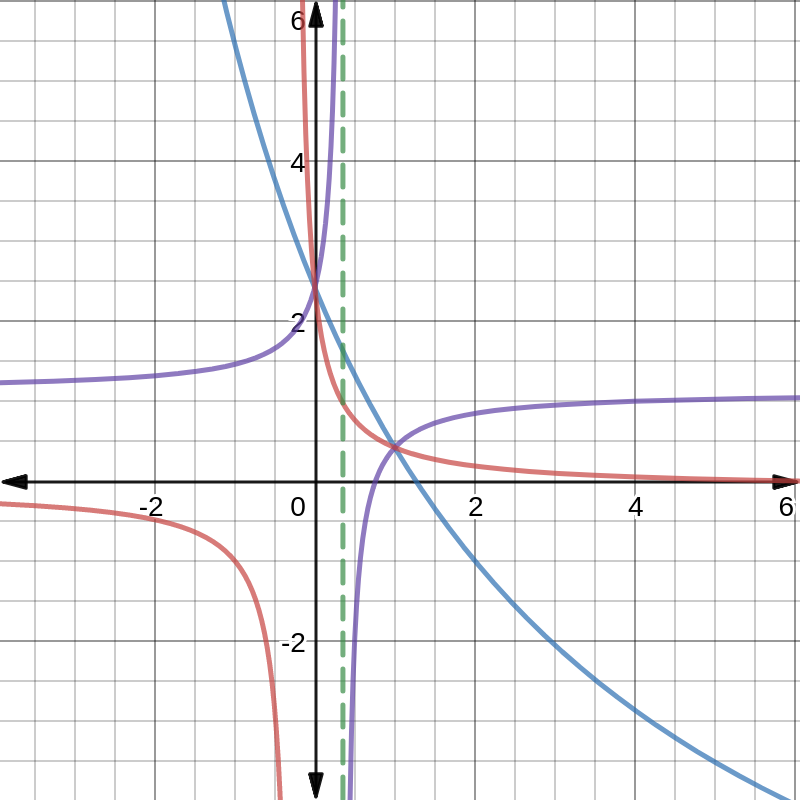
\includegraphics[scale=0.3]{images/graf_3_10}
  		\caption{Коэффициенты $k_A(\mu)$, $k_B(\mu)$ и $k(p,\mu)$ при фиксированном $p$}
		\label{fig:k_A,k_B,k}	
	\end{figure}	
	
	Рассмотрим график \ref{fig:k_A,k_B,k}, на котором изображены значения коэффициетов
	при фиксированном значении $p \in [0,1]$. $k_B(\mu)$ изображены красной кривой,
	$k_A(\mu)$ синей и фиолетовой - кривая $k(p, \mu)$. Пунктирная вертикальная линия
	обозначает точку $x$ в которой выражение $g_1=0$. Имеет место неравенство 
	$k_A(\mu) > k_B(\mu)$ при $\mu \in (0,1)$.
	
	$$
	\begin{cases}
	k(\mu) < k_B(\mu) \textrm{ при } g_1(\mu,p) < 0  \\
	k(\mu) > k_A(\mu) \textrm{ при } g_1(\mu,p) > 0 \\
	\end{cases}		
	$$	
	
	
	Следовательно точки максимума функции $\overline{G}(p,q,\mu)$ при фикисированных
	значениях $\mu$ и $p$ могут быть точки: 
	$\{A\}, \{B\}, (0,0)$ и отрезки $[B, A], [0, A], [0,B]$. Где точки
	$A(\mu)$ и $B(\mu)$ определны в \ref{eq:A} и \ref{eq:B}. 
	Рассмотрим три подслучая:
	
	\newpage

	\textbf{(a)} $0 \leqslant \mu \leqslant \frac{1}{3}$. 	
		
	\begin{figure}[H]
    	\centering
     	\begin{subfigure}[b]{0.3 \textwidth}
        	\centering
        	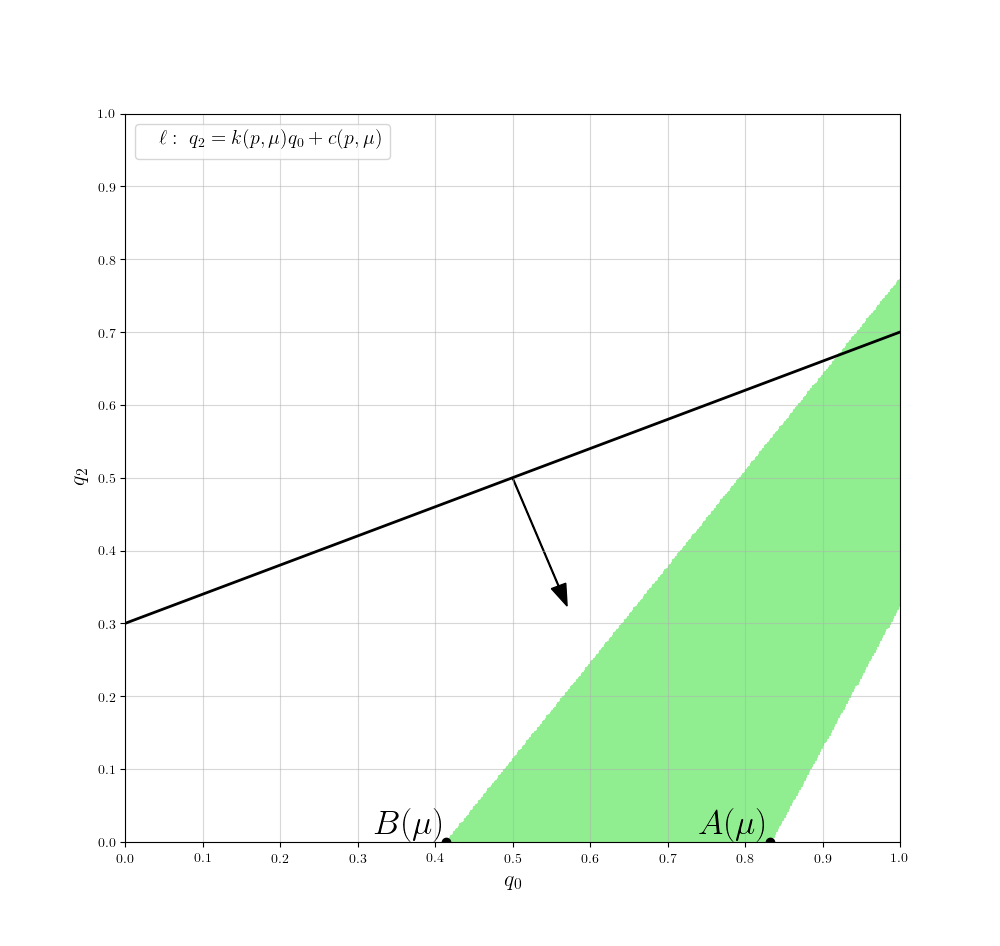
\includegraphics[width=\textwidth]{images/graf_3_9_0}
        	\caption{$g_1 > 0 \Rightarrow q^*=A$}
         	\label{fig:y equals x}
     	\end{subfigure}
     	\begin{subfigure}[b]{0.3 \textwidth}
        	\centering
        	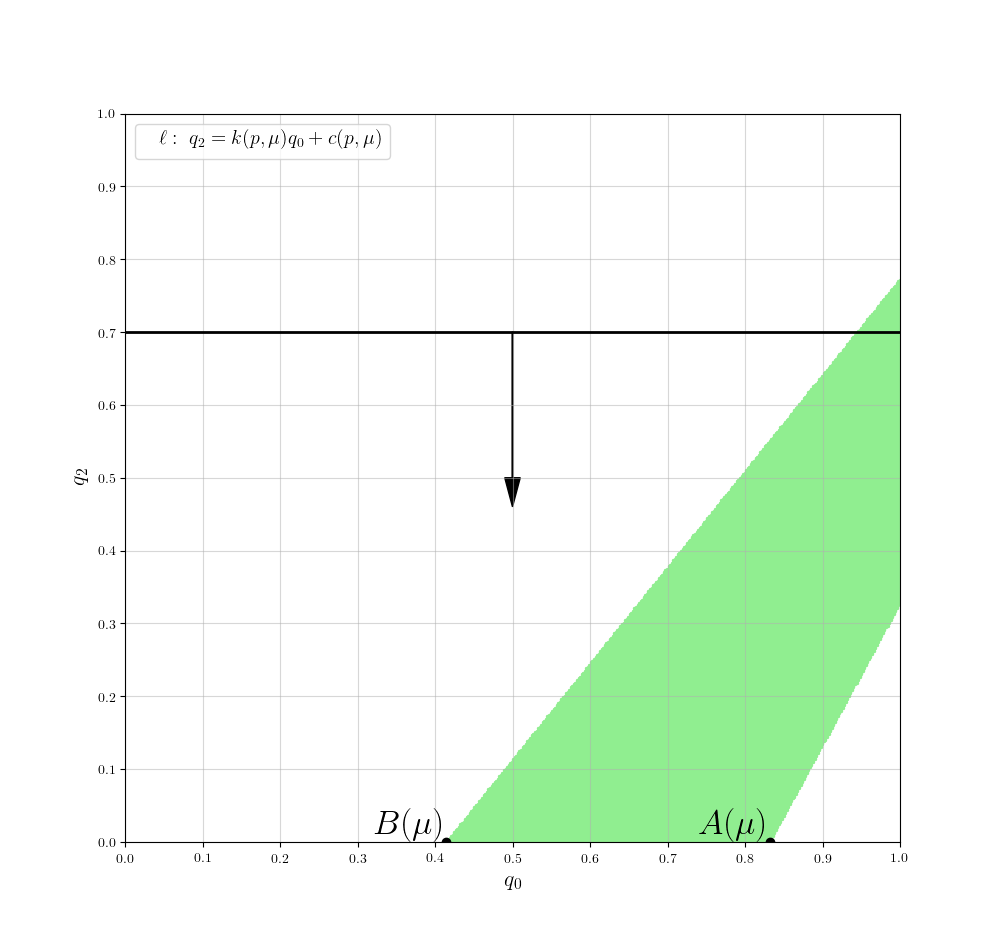
\includegraphics[width=\textwidth]{images/graf_3_9_2}
        	\caption{$g_1 = 0 \Rightarrow q^*=[B,A]$}
        	\label{fig:three sin x}
     	\end{subfigure}
     	\begin{subfigure}[b]{0.3 \textwidth}
        	\centering
        	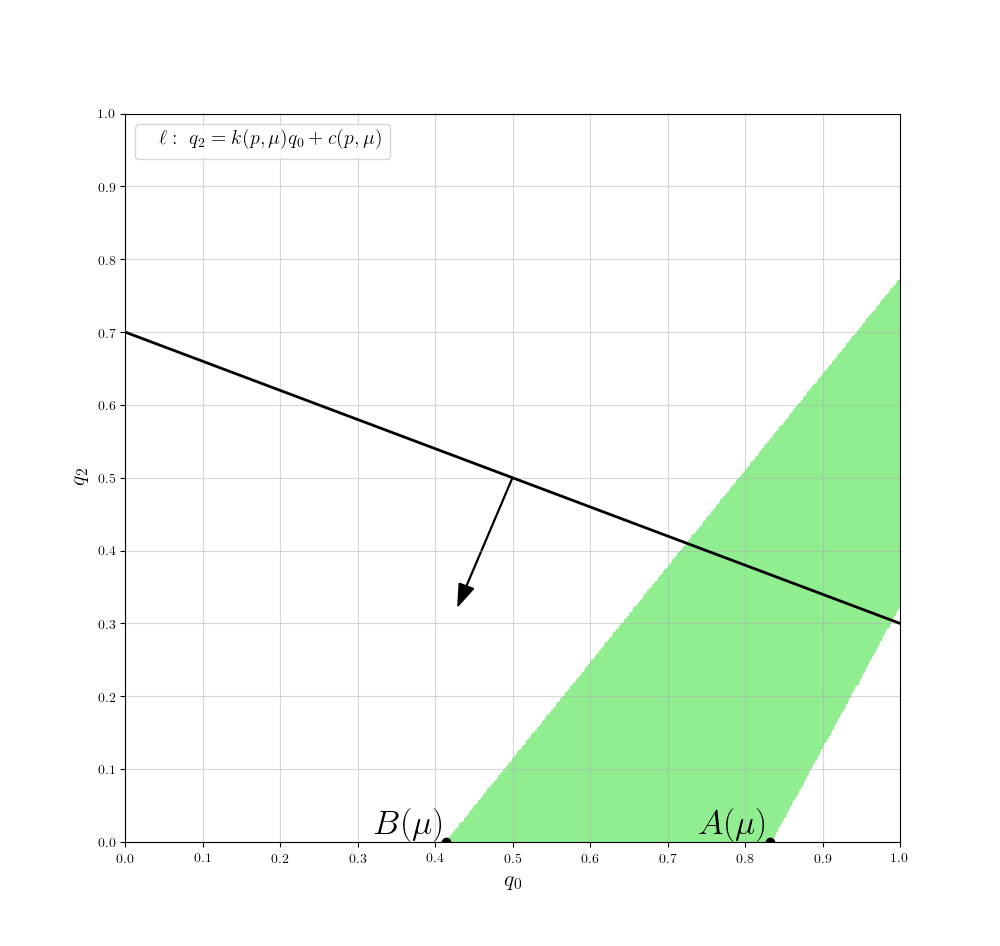
\includegraphics[width=\textwidth]{images/graf_3_9_1}
        	\caption{$g_1 < 0 \Rightarrow q^*=B$}
        	\label{fig:three sin x}
     	\end{subfigure}
     	\caption{}
     	\label{fig:3_mu_0}
	\end{figure}

	%Если наклон касательной меньше $k_A$ но больше нуля, то оптимальной точкой
	%является точка $A(\mu)$, если касатальеная паралельна оси $Oq_0$,
	%то множеству оптимальных точек соответсвует отрезок $[B,A]$, если же наклон
	%отрицательный то оптимальной точкой является точка $B(\mu)$.
	%Итого оптимальные точки соответсвуют следующей системе:	
	
	$$
		\begin{cases}
			g_1 > 0 \Rightarrow q^*=A \\
			g_1 = 0 \Rightarrow q^*=[B,A] \\
			g_1 < 0 \Rightarrow q^*=B
		\end{cases}
	$$	
	
	\textbf{(b)} $\frac{2}{3} \leqslant \mu \leqslant 1$
			
	\begin{figure}[H]
    	\centering
     	\begin{subfigure}[b]{0.3 \textwidth}
        	\centering
        	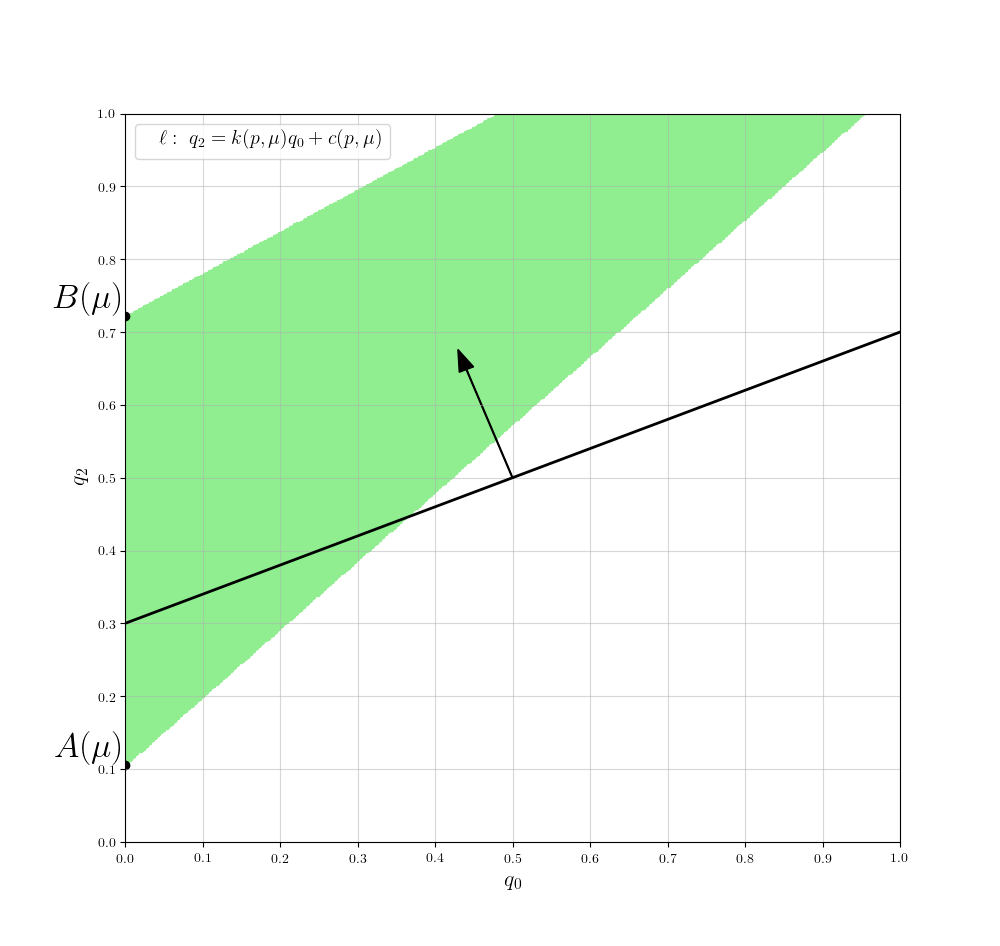
\includegraphics[width=\textwidth]{images/graf_3_7_0}
        	\caption{$g_2 > 0 \Rightarrow q^*=B$}
         	\label{fig:y equals x}
     	\end{subfigure}
     	\begin{subfigure}[b]{0.3 \textwidth}
        	\centering
        	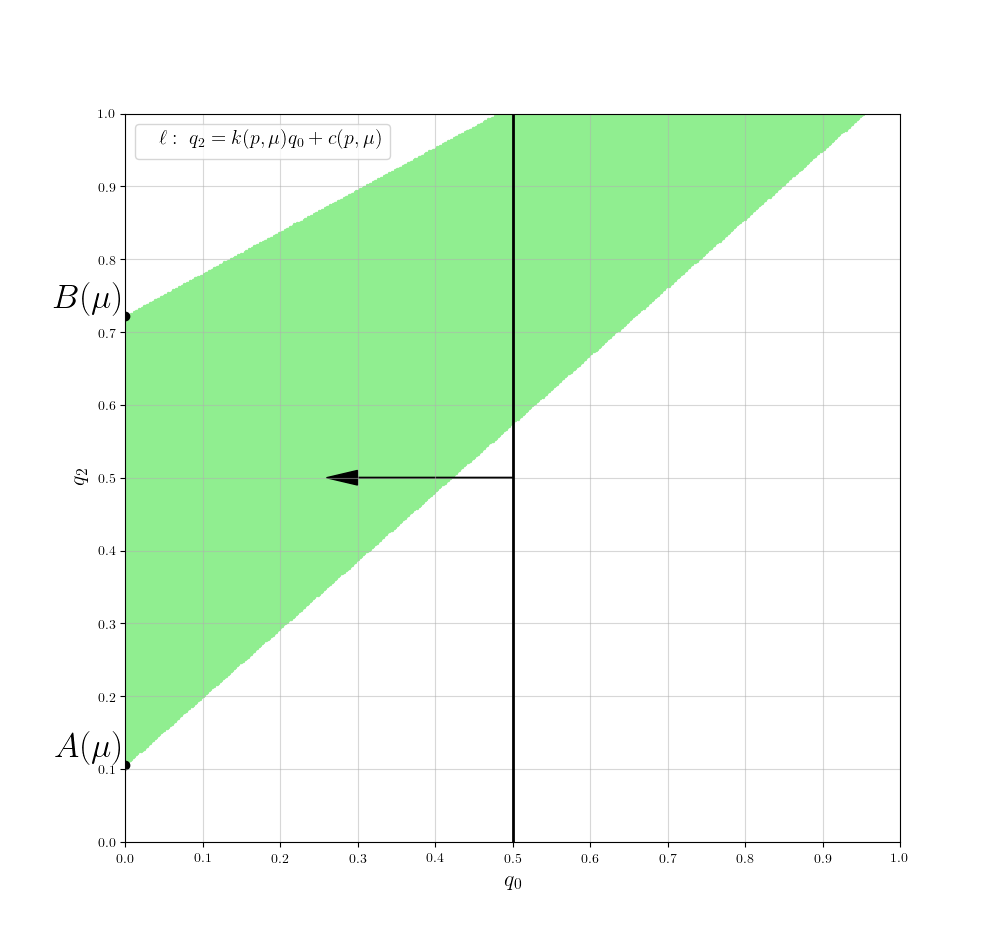
\includegraphics[width=\textwidth]{images/graf_3_7_1}
        	\caption{$g_2 = 0 \Rightarrow q^*=[B,A]$}
        	\label{fig:three sin x}
     	\end{subfigure}
     	\begin{subfigure}[b]{0.3 \textwidth}
        	\centering
        	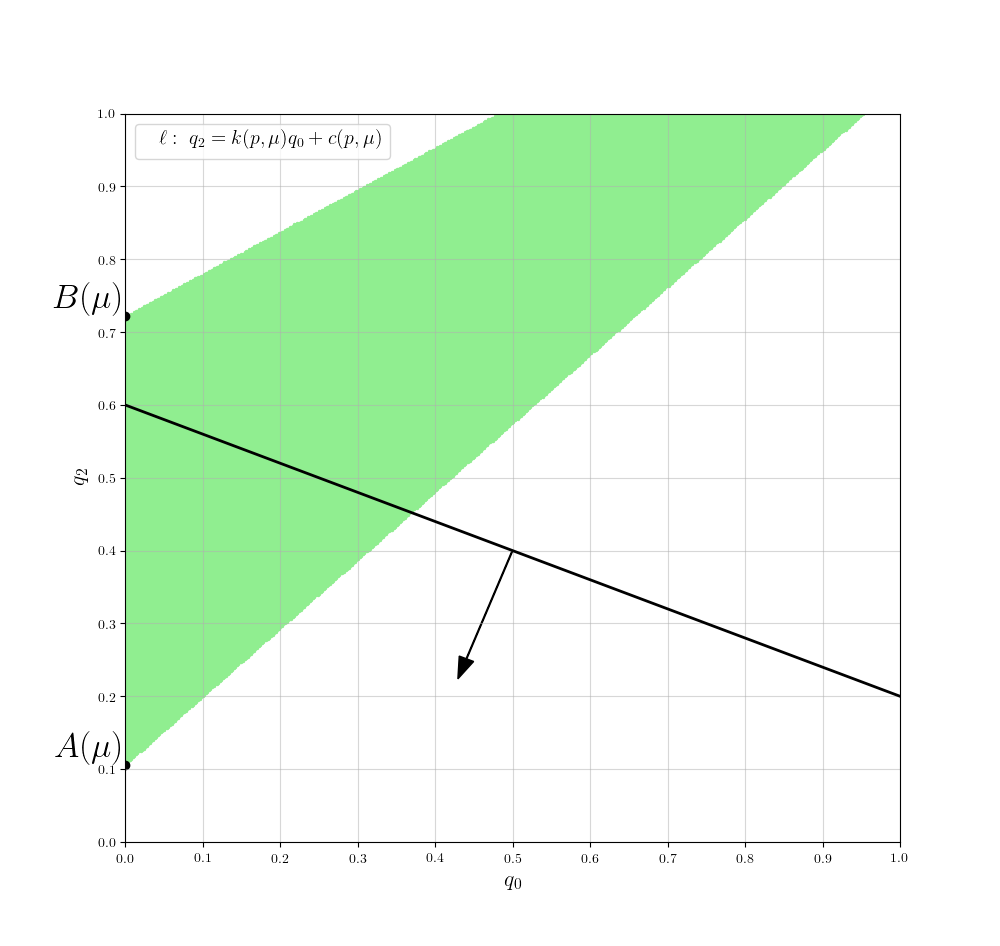
\includegraphics[width=\textwidth]{images/graf_3_7_2}
        	\caption{$g_2 < 0 \Rightarrow q^*=A$}
        	\label{fig:three sin x}
     	\end{subfigure}
     	\caption{}
	\end{figure}
	
	\begin{center}
		$\left[
		\begin{gathered}
			g_2 > 0 \Rightarrow q^*=B \\
			g_2 = 0 \Rightarrow q^*=[B,A] \\
			g_2 < 0 \Rightarrow q^*=A
		\end{gathered}
		\right.$	
	\end{center}	
	
	\newpage

	\textbf{(c)} $\frac{1}{3} \leqslant \mu \leqslant \frac{2}{3}$
	
	\begin{figure}[H]
    	\centering
     	\begin{subfigure}[b]{0.3 \textwidth}
        	\centering
        	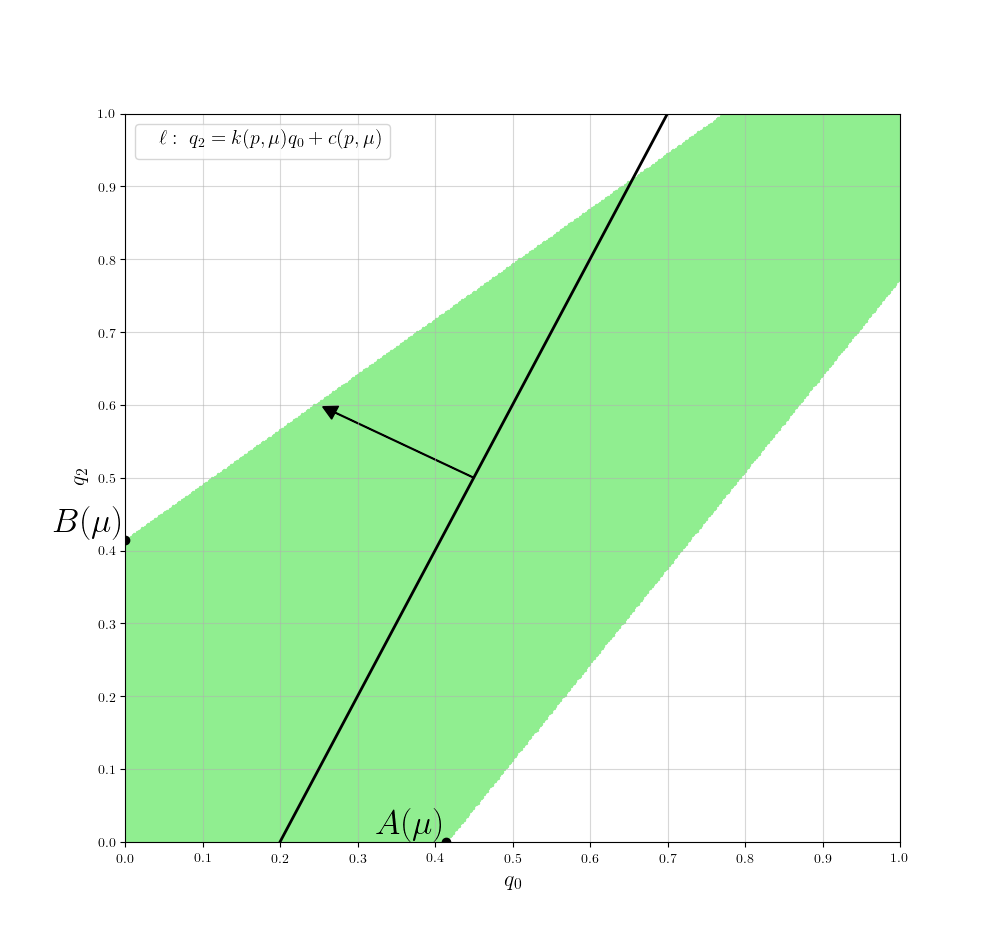
\includegraphics[width=\textwidth]{images/graf_3_8_1}
        	\caption{$g_2 > 0 \Rightarrow q^*=B$}
     	\end{subfigure}
     	\begin{subfigure}[b]{0.3 \textwidth}
        	\centering
        	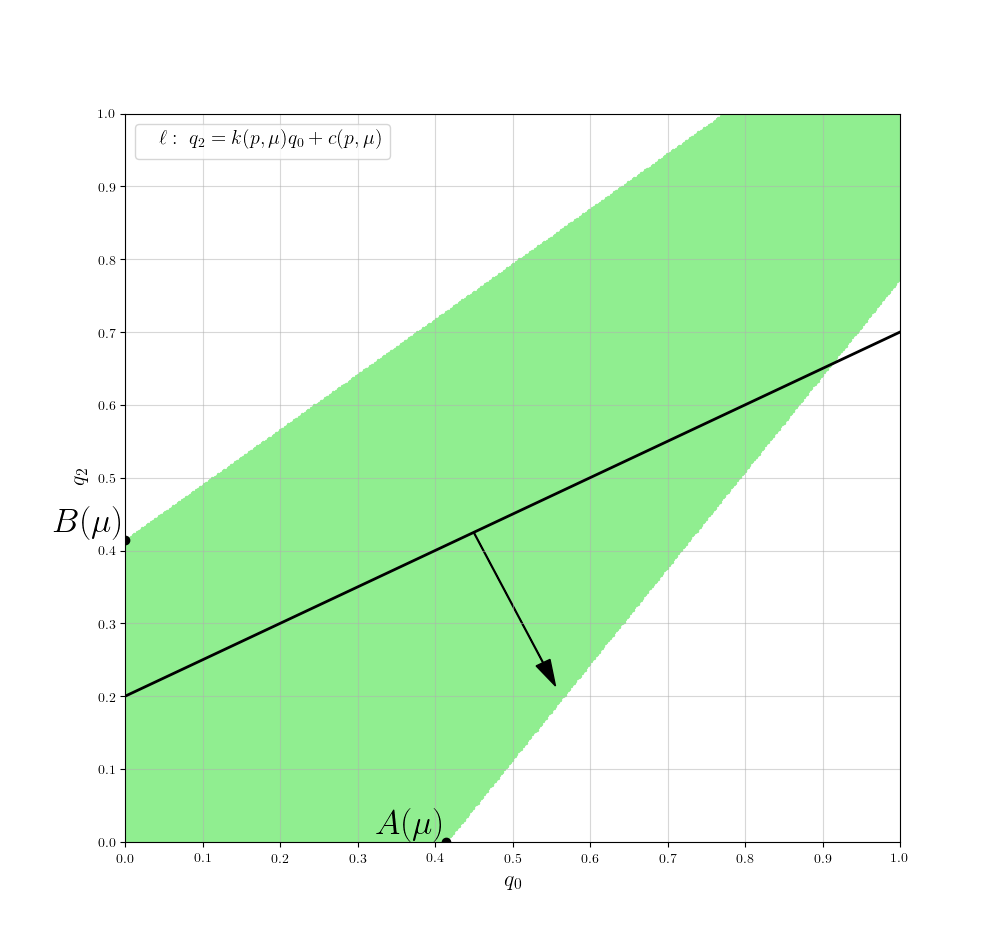
\includegraphics[width=\textwidth]{images/graf_3_8_2}
        	\caption{$g_1 > 0 \Rightarrow q^*=A$}
     	\end{subfigure}
     	\begin{subfigure}[b]{0.3 \textwidth}
        	\centering
        	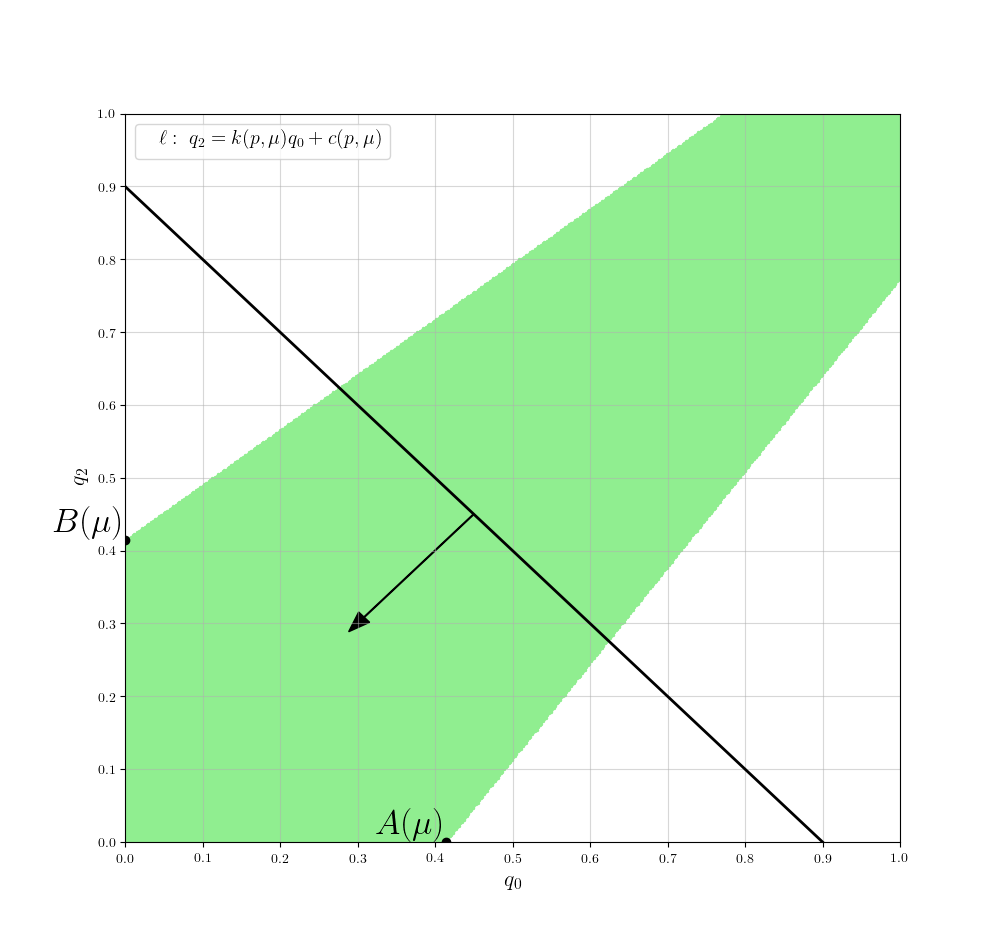
\includegraphics[width=\textwidth]{images/graf_3_8_0}
        	\caption{$
        	\begin{cases}			
				g_2 < 0 \\
				g_1 < 0
			\end{cases}	\Rightarrow q^*=(0,0)
			$}
     	\end{subfigure}
    	\centering
     	\begin{subfigure}[b]{0.3 \textwidth}
        	\centering
        	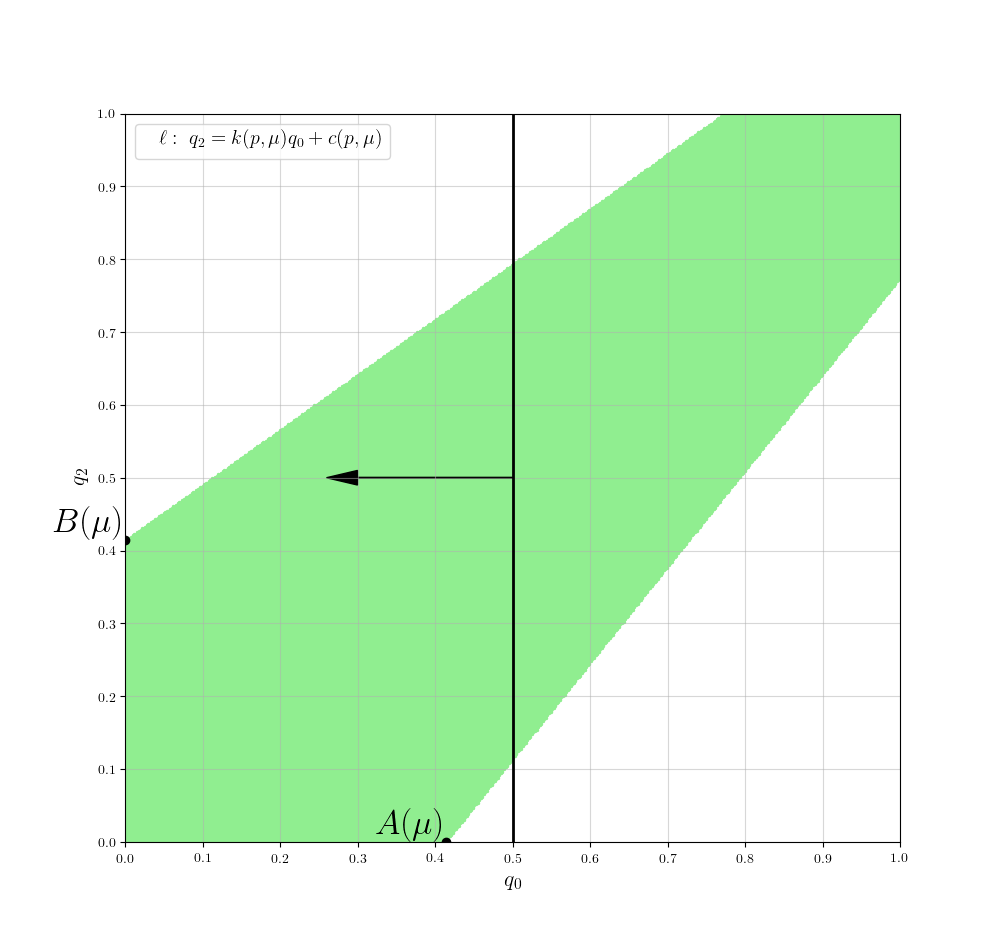
\includegraphics[width=\textwidth]{images/graf_3_8_3}
        	\caption{$g_2 = 0 \Rightarrow q^*=[0,B]$}
     	\end{subfigure}
     	\begin{subfigure}[b]{0.3 \textwidth}
        	\centering
        	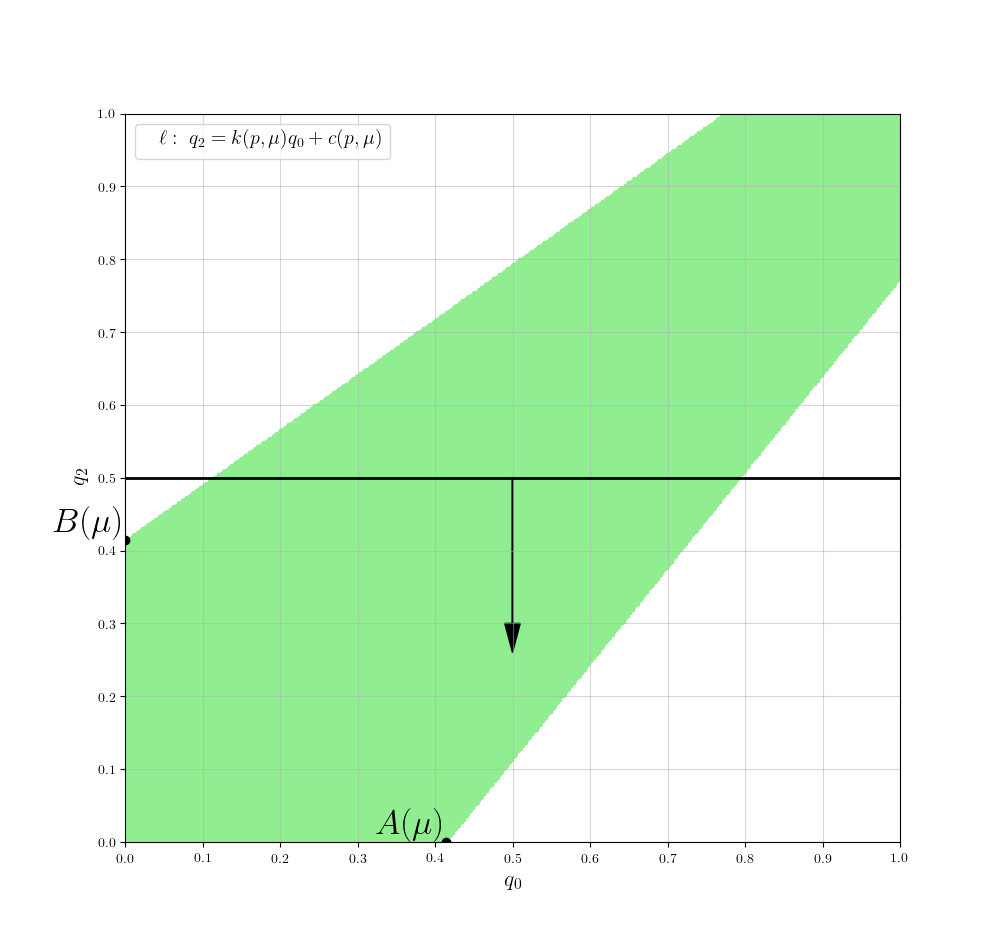
\includegraphics[width=\textwidth]{images/graf_3_8_4}
        	\caption{$g_1 = 0 \Rightarrow q^*=[0,A]$}
     	\end{subfigure}
	\end{figure}


	
	\begin{center}
		$\left[
		\begin{gathered}
			g_1 > 0 \Rightarrow q^*=A \\
			g_2 > 0 \Rightarrow q^*=B \\			
			g_1 = 0 \Rightarrow q^*=[0,A] \\
			g_2 = 0 \Rightarrow q^*=[0,B] \\			
			\begin{cases}			
				g_2 < 0 \\
				g_1 < 0
			\end{cases}	\Rightarrow q^*=(0,0)
		\end{gathered}
		\right.$	
	\end{center}

%-------------------------------------------------------------

	Итого получим следующие 

	$C(p,\mu) = \arg \max \limits_{P_{AB}} \overline{G}(p,q,\mu)
	\begin{cases}
	A(\mu), & g_2(p,\mu)<0 \cup \mu \leqslant \frac{1}{3} \cap g_2 < 0 \\
	B(\mu), & g_1(p,\mu)>0 \cup \mu \geqslant \frac{2}{3} \cap g_1 > 0 \\
	(0,0),  & g_1(p,\mu)<0 \cap g_2(p,\mu)<0 \\
	[A(\mu), B(\mu)], 
	& g_1(\mu)=0 \cap \mu < \frac{1}{3} \cup g_1(\mu)=0 \cap \mu > \frac{2}{3} \\
	[0, A(\mu)], & g_2(\mu)=0 \cap \mu \in [\frac{1}{3},\frac{2}{3}] \\
	[0, B(\mu)], & g_1(\mu)=0 \cap \mu \in [\frac{1}{3},\frac{2}{3}] \\
	\end{cases}	
	$	
	
	Но кроме того точки $A(\mu)$ и $B(\mu)$ являются оптимальными 
	$\forall$ $p$ и $\mu$ поскольку	являются таковыми в \textbf{(1)} и \textbf{(2)}.
	Итого в области $P_B$ оптимальной является точка $B(\mu)$,
	в области $P_A$ оптимальной является точка $A(\mu)$,
	и в области $P_{AB}$ оптимальной является точка $C(p, \mu)$.
	Поскольку если $f(x)$ и $g(x)$ непрерывны на множестве $X$, то и 
	$min(f(x), g(x))$ непрерывна на $X$, то максимум достигается в точке
	$C$.
	
	$q^*(p,\mu)= \arg \max \limits_Q \overline{G}(p,q,\mu)
	\begin{cases}
	A(\mu), & g_2(p,\mu)<0 \cup \mu \leqslant \frac{1}{3} \cap g_2 < 0 \\
	B(\mu), & g_1(p,\mu)>0 \cup \mu \geqslant \frac{2}{3} \cap g_1 > 0 \\
	(0,0),  & g_1(p,\mu)<0 \cap g_2(p,\mu)<0 \\
	[A(\mu), B(\mu)], 
	& g_1(\mu)=0 \cap \mu < \frac{1}{3} \cup g_1(\mu)=0 \cap \mu > \frac{2}{3} \\
	[0, A(\mu)], & g_2(\mu)=0 \cap \mu \in [\frac{1}{3},\frac{2}{3}] \\
	[0, B(\mu)], & g_1(\mu)=0 \cap \mu \in [\frac{1}{3},\frac{2}{3}] \\
	(0,1), & \mu = 0 \\
	(1,0), & \mu = 1
	\end{cases}	
	$		
	
	
	%$$g_1=p\mu-(1-p)(1-\mu)  \hspace{10mm}
	%g_1=0 \sim p=\frac{1-\mu}{(\sqrt{2}-2)\mu + 1}$$

	%$$g_2=(1-p)(1-\mu)(\sqrt{2}-1)-p\mu  \hspace{10mm}
	%g_2=0 \sim p=\frac{(1-\mu)(\sqrt{2}-1)}{(\sqrt{2}-2)\mu + (\sqrt{2}-1)}$$
	
	Поскольку в пункте 3.1 мы установили, что 
	
	$$p^*(q,\lambda(q))=\arg \max \limits_{p \in [0,1]}
		\overline{L}(p, q, \lambda(q))=[0,1]
	$$

	Нас интересуют оптимальные пары $(p^0,q^0)$ такие, что 
	$\exists (\lambda, \mu) \in [0,1]^2 $:
	
	$$\begin{cases}
	p^0=p^*(q^0,\lambda) \\
	q^0=q^*(p^0,\mu)
	\end{cases}$$
	
	Введём следующие множества:
	
	$$P_0=[0,1], \; Q_0=\{(q_0,q_2) \in Q \: | \: q_0=0 \textrm{ или } q_2 = 0\}$$
	
	Следующие точки являются оптимальными:
	$$(p, q) \in P_0 \times Q_0$$
		

\end{flushleft}




















%\section{Оптимальные значения}

\subsection{Заключение}
\begin{flushleft}
	Заключение
\end{flushleft}

\newpage
\bibliographystyle{plain}
\bibliography{include/bibliogaphy}

%\include{Chapter1} % Введение
%\include{Chapter2} % Постановка задачи
%\include{Chapter3} % Решение задачи
%\include{Chapter4} % Задача с неопределенностью
%\include{Chapter5} % Список литературы


%\nocite{*}
%\bibliographystyle{gost71u} % Для соответствия требованиям об %оформлении списка литературы
%\bibliography{references}

% \include{Appendix} 

\end{document}
